\chapter{Casos de estudio y validación}
\label{ch:casos_estudio}

\section{Rol de los casos de estudio en la tesis}

La validación de \hydra requiere demostrar que los módulos implementados producen resultados coherentes con datos observados y con estudios previos, y que el flujo integrado reduce la carga manual sin comprometer la calidad técnica del análisis. Los casos de estudio que se presentan en este capítulo no son aplicaciones paralelas a la tesis, sino el sustrato empírico sobre el que se han construido los módulos y desde el que se han tomado las decisiones de diseño.

Cada caso cubre una combinación distinta de escalas espaciales, regímenes hidrológicos, modelos físicos y técnicas estadísticas. Esta diversidad es deliberada: permite comprobar que los módulos son suficientemente generales y que las convenciones de datos y las interfaces entre bloques funcionan en contextos reales. La existencia de publicaciones asociadas a cada caso proporciona una referencia externa independiente para verificar resultados.

La validación se estructura en dos niveles de naturaleza distinta. A nivel de módulo, la comprobación se apoya en los notebooks de ejemplo, que reproducen resultados de referencia (ajustes publicados, datos sintéticos con solución conocida, modelos oficiales de prueba de cada motor) y actúan como tests ejecutables de cada funcionalidad; la consolidación de estas comprobaciones en una suite de tests automáticos con cobertura de integración entre bloques es una tarea en curso que se recoge en el trabajo futuro (\cref{ch:conclusiones}). A nivel de flujo, que es el que este capítulo documenta con detalle, se verifica que la cadena completa, desde la obtención de datos hasta la generación de productos de riesgo, produce resultados interpretables, reproducibles y comparables con estudios previos publicados.

Los nueve casos no son una colección heterogénea de trabajos: cada uno valida dimensiones específicas de \hydra y en conjunto cubren la totalidad de los módulos principales. Para clarificar qué valida cada caso y evitar que la amplitud de la selección se interprete como dispersión metodológica, la \cref{tab:grupos_validacion} los clasifica en tres grupos de validación.

\begin{table}[htbp]
  \centering
  \caption{Clasificación de los nueve casos de estudio por grupo de validación y dimensión que cubren.}
  \label{tab:grupos_validacion}
  \small
  \begin{tabular}{p{0.25\textwidth}p{0.28\textwidth}p{0.35\textwidth}}
    \toprule
    Grupo & Casos & Qué validan \\
    \midrule
    \textbf{Núcleo de inundación estocástica basada en impacto} & Besaya, Sant Llorenç des Cardassar, Calle 30 & Cópulas multivariantes, generación de escenarios, selección MaxDiss, adaptadores de modelos hidráulicos integrados en \pyhydra (HEC-HMS, HEC-RAS, SFINCS) --- con Iber como motor hidráulico usado manualmente en las aplicaciones iniciales, sin adaptador de automatización ---, reconstrucción k-NN, período de retorno sobre impacto \\[6pt]
    \textbf{Incertidumbre estadística y extremos} & Valencia DANA 2024 & Comparación de estimadores GEV (MLE, L-momentos, bayesiano), análisis de frecuencia regional, comportamiento ante eventos sin precedente histórico \\[6pt]
    \textbf{Cambio climático, datos globales y escalabilidad} & Lago Tanganica, vulnerabilidad hidroeléctrica andina, cuenca atlántica--IAHR 2022, SIMPCCe, Atlas de Panamá & Descarga automática de ERA5/CMIP6, corrección de sesgo, proyecciones multi-modelo, escalabilidad a dominios nacionales y contextos con datos escasos \\
    \bottomrule
  \end{tabular}
\end{table}

La selección evita duplicar el contenido completo de los artículos ya publicados en revistas. En esos casos se sintetiza únicamente la aplicación y su relación con \hydra. Las comunicaciones presentadas en congresos y los proyectos técnicos se documentan con mayor detalle porque muestran etapas intermedias de desarrollo, decisiones de implementación y productos gráficos que no siempre quedaron recogidos en las publicaciones posteriores. La \cref{tab:casos_fuentes} identifica la procedencia principal de las aplicaciones documentadas con material de congresos o proyectos.

\begin{longtable}{p{0.20\textwidth}p{0.32\textwidth}p{0.33\textwidth}}
  \caption{Procedencia documental de los casos de estudio empleados para validar \hydra. Cada fila incluye la referencia bibliográfica o técnica empleada como fuente principal.}
  \label{tab:casos_fuentes} \\
  \toprule
  Caso & Difusión principal & Papel en el capítulo \\
  \midrule
  \endfirsthead
  \toprule
  Caso & Difusión principal & Papel en el capítulo \\
  \midrule
  \endhead
  Besaya--Los Corrales de Buelna & Aplicación fundacional de 2018 \parencite{navas2018besaya}; análisis de sensibilidad hidráulica Monte Carlo \parencite{navas2025roughness}; Iber como motor hidráulico inicial \parencite{blade2014iber} & Origen de la cadena estocástica basada en impactos y banco de pruebas para automatización y sensibilidad hidráulica. \\
  Sant Llorenç des Cardassar, Mallorca & VI Jornadas de Ingeniería del Agua, 2019 \parencite{navas2019mallorca}; productos satelitales de apoyo PERSIANN/TRMM \parencite{ashouri2015persiann,huffman2007trmm}; referencia hidráulica Iber \parencite{blade2014iber} & Primer downscaling híbrido desde lluvia: satélite como diagnóstico, kriging pluviométrico, selección MaxDiss, simulación y reconstrucción k-NN. \\
  Calle 30, Madrid & VII Jornadas de Ingeniería del Agua, 2023 \parencite{deljesus2023calle30}; artículo de caso \parencite{navas2024calle30}; formulación de downscaling híbrido \parencite{deljesus2024downscaling} & Aplicación urbana integrada de la metodología estocástica basada en precipitación multisitio, HEC-HMS y HEC-RAS 1D. \\
  Valencia: episodio DANA octubre 2024 & VIII Jornadas de Ingeniería del Agua, 2025 \parencite{deljesus2025jia}; EGU General Assembly 2025 \parencite{deljesus2025valencia}; artículo enviado \parencite{navas2025valenciaIA} & Comparación de métodos GEV (MLE, L-momentos, MCMC) y análisis de frecuencia regional sobre un evento sin precedente histórico. \\
  Lago Tanganica & VIII Jornadas de Ingeniería del Agua, 2025 \parencite{navas2025tanganika}; artículo enviado \parencite{navas2025tanganicaIA}; base climática ERA5/CMIP6 \parencite{hersbach2020era5,eyring2016cmip6} & Estimación de niveles de diseño bajo cambio climático combinando ERA5, CMIP6, altimetría satelital y aprendizaje automático. \\
  Vulnerabilidad hidroeléctrica en los Andes & VI Jornadas de Ingeniería del Agua, 2019 \parencite{deljesus2019andean}; escenarios regionales de cambio climático derivados de CORDEX/CMIP & Procesamiento climático regional, interpolación espacial y modelización hidrológica distribuida. \\
  Cuenca atlántica -- decisiones metodológicas (IAHR 2022) & 39th IAHR World Congress \parencite{deljesus2022iahr}; base metodológica de corrección de sesgo \parencite{teutschbein2012biascorrection}; Iber \parencite{blade2014iber} & Cuantificación sistemática del error de la metodología estándar frente a la estocástica bajo escenarios de cambio climático. \\
  SIMPCCe & VII Jornadas de Ingeniería del Agua, 2023 \parencite{navas2023simpce}; IAHR Europe, 2024 \parencite{navas2024iahrsimpcce}; artículo posterior \parencite{navas2025simpce} & Transferencia de los módulos climáticos a una aplicación operativa de recursos hídricos y planificación. \\
  Atlas de Riesgo Climático de Panamá & Proyecto Ministerio de Ambiente--BID \parencite{ihcantabria2023panama}; base climática global ERA5/CMIP6 \parencite{hersbach2020era5,eyring2016cmip6}; SFINCS \parencite{leijnse2021sfincs} & Descarga e interpolación climática nacional, corrección de sesgo masiva y ejecución sistemática de SFINCS a escala de país. \\
  \bottomrule
\end{longtable}

\begin{landscape}
\begingroup
\footnotesize
\setlength{\tabcolsep}{4pt}
\begin{longtable}{>{\raggedright\arraybackslash\hspace{0pt}}p{0.11\linewidth}>{\raggedright\arraybackslash\hspace{0pt}}p{0.19\linewidth}>{\raggedright\arraybackslash\hspace{0pt}}p{0.23\linewidth}>{\raggedright\arraybackslash\hspace{0pt}}p{0.25\linewidth}>{\raggedright\arraybackslash\hspace{0pt}}p{0.11\linewidth}}
  \caption{Matriz de validación de \hydra por caso de estudio, módulo, evidencia reproducible y criterio de aceptación.}
  \label{tab:matriz_validacion_hydra} \\
  \toprule
  Caso & Módulos de \hydra ejercitados & Evidencia de validación & Criterio de aceptación & Limitación principal \\
  \midrule
  \endfirsthead
  \toprule
  Caso & Módulos de \hydra ejercitados & Evidencia de validación & Criterio de aceptación & Limitación principal \\
  \midrule
  \endhead
  Besaya--Los Corrales de Buelna &
  Extracción de eventos, cópulas, adaptadores hidráulicos, postprocesado espacial, sensibilidad de Manning &
  Publicación fundacional \parencite{navas2018besaya}, artículo de sensibilidad hidráulica \parencite{navas2025roughness} y notebooks internos de análisis del ensemble &
  Reproducción de la lógica de período de retorno sobre impacto; comparación emparejada de 995 simulaciones SFINCS--HEC-RAS; identificación trazable de bifurcación hidráulica y variabilidad intermodelo &
  Parte del material es interno y depende de modelos hidráulicos externos \\[5pt]

  Sant Llorenç des Cardassar &
  Reconstrucción espacial de precipitación, cópulas multisitio, MaxDiss, Iber, reconstrucción k-NN &
  Comunicación JIA \parencite{navas2019mallorca}, mancha Copernicus del episodio histórico y notebook interno de reconstrucción de precipitación &
  Coherencia espacial de la lluvia reconstruida; reproducción razonable de la mancha observada; reducción del número de simulaciones mediante selección representativa sin perder cobertura del espacio de eventos &
  Series cortas y ausencia de aforos locales \\[5pt]

  Calle 30--M-30 &
  ERA5/AEMET, extremos de precipitación, cópulas multivariantes, HEC-HMS, HEC-RAS 1D, MaxDiss, k-NN, período de retorno por píxel &
  Comunicación JIA \parencite{deljesus2023calle30}, artículos asociados \parencite{navas2024calle30,deljesus2024downscaling} y notebooks de flujo hidrológico-hidráulico &
  Obtención de mapas de calado por período de retorno; diferencia cuantificada entre frecuencia del forzamiento y frecuencia del impacto; ejecución encadenada de lluvia, hidrología, hidráulica y reconstrucción &
  Geometría urbana y configuración HEC-RAS \\[5pt]

  Valencia DANA 2024 &
  Descarga de observaciones, GEV por MLE/L-momentos/MCMC, análisis de frecuencia regional, cuantificación de incertidumbre &
  Comunicación JIA \parencite{deljesus2025jia}, resumen EGU \parencite{deljesus2025valencia}, artículo enviado \parencite{navas2025valenciaIA} y notebook de extremos del caso Valencia &
  Comparación reproducible de estimadores con y sin el evento; sensibilidad explícita de los períodos de retorno; intervalos bayesianos y contraste regional frente a estaciones próximas &
  Evento reciente y series con cola distribucional poco informada \\[5pt]

  Lago Tanganica &
  ERA5/CMIP6, corrección de sesgo delta, regresión ML, bootstrap de residuos, extremos no paramétricos &
  Comunicación JIA \parencite{navas2025tanganika}, artículo enviado \parencite{navas2025tanganicaIA}, altimetría Hydroweb y notebooks de cambio climático &
  Reconstrucción de niveles con ajuste histórico verificable; propagación de incertidumbre intermodelo; estimación de cotas de diseño bajo SSP2-4.5 y SSP5-8.5 &
  Escasez de observaciones instrumentales continuas \\[5pt]

  Andes hidroeléctricos &
  Interpolación climática, corrección de sesgo, procesamiento regional y modelización hidrológica distribuida &
  Comunicación JIA \parencite{deljesus2019andean}, calibración hidrológica y validación cruzada de campos climáticos &
  Correlación y sesgo documentados en interpolación; calibración VIC con NSE y PBIAS; ejecución regional sobre cuatro países y múltiples modelos climáticos &
  Redes nacionales heterogéneas y cobertura amazónica limitada \\[5pt]

  Cuenca atlántica--IAHR 2022 &
  Corrección de sesgo EURO-CORDEX, cópulas, MaxDiss, Iber, reconstrucción k-NN, comparación de metodologías &
  Comunicación IAHR \parencite{deljesus2022iahr} y comparación sistemática estándar--estocástica &
  Diferencias de caudal de diseño del 30--37\% entre metodología estándar y estocástica; demostración de que la discrepancia espacial no se corrige con un factor uniforme &
  Caso centrado en una cuenca y motores concretos \\[5pt]

  SIMPCCe &
  Descarga climática nacional, corrección de sesgo SDM, ANN, análisis de sequía e informes automáticos &
  Guía metodológica de Fundación Canal \parencite{fundacioncanal2022guiaembalses}, comunicaciones JIA/IAHR Europe \parencite{navas2023simpce,navas2024iahrsimpcce}, artículo \parencite{navas2025simpce} y Premio al Talento Joven ``M.R. Llamas'' del Observatorio del Agua de la Fundación Botín &
  Reutilización de módulos climáticos en una aplicación industrial; generación sistemática de 60 series corregidas por variable y síntesis automática para toma de decisiones &
  Orientado a recursos hídricos, no a inundación hidráulica directa \\[5pt]

  Atlas de Panamá &
  ERA5, TRMM y CMIP6; NEOPRENE (NSRP/STNSRP); kriging nacional; SDM/QDM; GEV; SFINCS; productos web &
  Memoria técnica del Atlas \parencite{ihcantabria2023panama}, visor web institucional y ejecución nacional de capas de amenaza &
  Escalado a 52 cuencas, 23 modelos CMIP6, 414 correcciones de sesgo y miles de simulaciones SFINCS; publicación de capas en un producto operativo para administración pública &
  Datos nacionales heterogéneos y dependencia de infraestructura de cálculo \\[5pt]

  Web y notebooks de \hydra &
  Todos los bloques funcionales: datos, clima, análisis espacial, generación estocástica, modelos y postprocesado &
  Interfaz web descrita en la \cref{sec:interfaz_web}, 26 notebooks generales inventariados en el \cref{app:notebooks}, 23 entradas de casos piloto en el catálogo web y entorno Docker/JupyterLab &
  Los notebooks documentan llamadas a la API, entradas, salidas y contratos funcionales de módulo; la web permite recorrer y lanzar los flujos desde un catálogo único, separando ejemplos generales de casos piloto &
  Validación funcional complementaria, no sustituto de la validación territorial \\
  \bottomrule
\end{longtable}
\endgroup
\end{landscape}

La \cref{tab:matriz_validacion_hydra} separa tres tipos de evidencia. Las publicaciones y comunicaciones proporcionan contraste científico externo; los proyectos industriales demuestran transferencia a contextos reales de ingeniería; y la web de \hydra, junto con los notebooks reproducibles, muestra que los módulos no solo existen en el código, sino que pueden ejecutarse siguiendo flujos documentados. Esta última capa es especialmente relevante en una tesis industrial: la validación no se limita al resultado científico de cada caso, sino que incluye la capacidad de convertir esos métodos en un producto técnico navegable, ejecutable y mantenible.

\section{Río Besaya, Los Corrales de Buelna}
\label{sec:caso_besaya}

\subsection{Contexto y problema}

El río Besaya, en Cantabria, discurre por Los Corrales de Buelna en una llanura de inundación con actividad industrial y residencial significativa. El régimen hidrológico atlántico de la cuenca genera episodios de crecida asociados a frentes de larga duración con intensidades moderadas pero elevados volúmenes acumulados. En estas condiciones, la caracterización del riesgo de inundación requiere representar adecuadamente la distribución conjunta de pico, volumen y duración de la avenida, que no pueden tratarse como variables independientes \parencite{navas2018besaya}.

\begin{figure}[htbp]
  \centering
  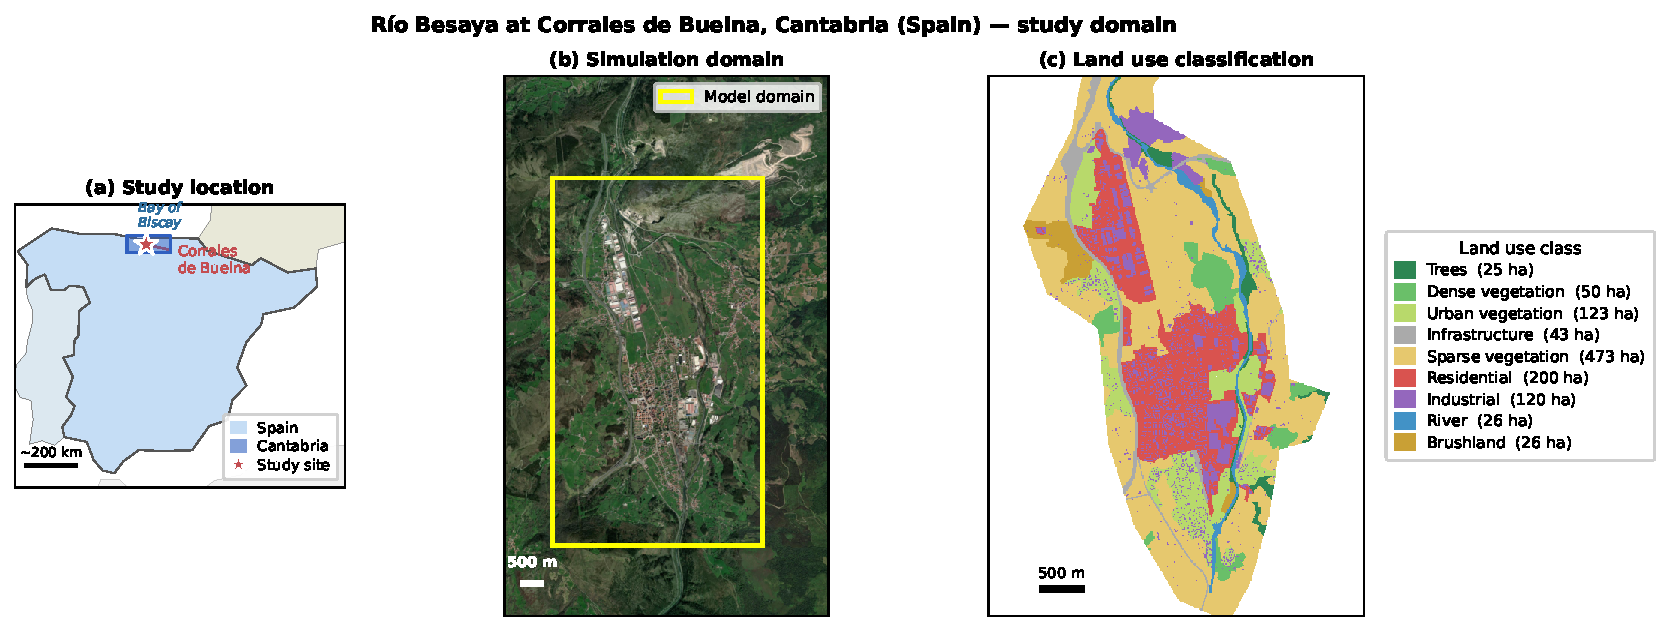
\includegraphics[width=\textwidth]{figures/besaya_fig00_location_map.pdf}
  \caption{Localización del área de estudio del río Besaya en Los Corrales de Buelna (Cantabria). Se muestran el tramo de análisis en la llanura de inundación, las secciones de aforo empleadas y el dominio de la malla hidráulica. Fuente: \parencite{navas2025roughness}.}
  \label{fig:besaya_localizacion}
\end{figure}

Este fue el caso inicial de la línea de investigación y el origen conceptual de \hydra. El trabajo de 2018 planteó, en el contexto de la línea de investigación, la cadena completa que desplaza el período de retorno desde el forzamiento hacia el impacto: generar muchos eventos hidrológicamente plausibles, propagarlos por modelos hidrológicos e hidráulicos y estimar la frecuencia sobre los calados y extensiones resultantes. La necesidad de repetir de forma consistente la preparación de entradas, las ejecuciones y el postprocesado reveló desde el inicio que el principal obstáculo no era un algoritmo aislado, sino la ausencia de una infraestructura reproducible que conectase todas las etapas.

\subsection{Metodología aplicada}

A diferencia del caso Mallorca, la aplicación inicial del Besaya parte de series de aforo. A partir de los registros de caudal se extraen eventos independientes y se caracterizan mediante caudal pico ($Q_p$), duración y volumen. Esta representación multivariante se eligió porque dos avenidas con el mismo pico pueden producir impactos distintos si difieren en volumen o persistencia; asignar toda la frecuencia al pico ocultaría esa diferencia.

La dependencia entre las tres variables se modela con una cópula gaussiana, con marginales ajustadas individualmente. El muestreo amplía el registro observado con eventos sintéticos que conservan combinaciones plausibles de pico, duración y volumen. En el trabajo de 2018, los hidrogramas de diseño se transformaron en manchas y calados mediante Iber, que fue el motor hidráulico empleado en la publicación de la \textit{Revista de Obras Públicas} \parencite{navas2018besaya}. La automatización de HEC-RAS aparece en trabajos posteriores, especialmente en Calle 30 y en el análisis de sensibilidad hidráulica desarrollado posteriormente sobre el mismo dominio.

Cada bloque responde a una limitación concreta y después se generaliza en \hydra: \texttt{climate.time\_series} estandariza la extracción de eventos; \texttt{spatial\_analysis.copulas} evita combinaciones multivariantes incoherentes; los adaptadores de modelos reducen la edición manual entre ejecuciones; y \texttt{hybrid\_downscaling} reduce el coste mediante selección por máxima disimilitud y reconstrucción k-NN. El producto final no es un único mapa determinista, sino una distribución de calado por celda a partir de la que se calculan niveles de retorno.

\begin{figure}[!htbp]
\centering
\resizebox{\textwidth}{!}{%
\begin{tikzpicture}[
  font=\scriptsize,
  proc/.style={
    rectangle, rounded corners=5pt,
    minimum width=2.9cm, minimum height=0.92cm,
    text width=2.65cm, align=center,
    draw=#1!60!black, fill=#1!11,
    line width=0.65pt
  },
  data/.style={
    rectangle, rounded corners=5pt,
    minimum width=2.75cm, minimum height=0.78cm,
    text width=2.5cm, align=center,
    draw=blueblock!65!black, fill=blueblock!10,
    line width=0.6pt
  },
  terrain/.style={
    rectangle, rounded corners=5pt,
    minimum width=2.75cm, minimum height=0.78cm,
    text width=2.5cm, align=center,
    draw=orangeblock!70!black, fill=orangeblock!14,
    line width=0.6pt
  },
  result/.style={
    rectangle, rounded corners=5pt,
    minimum width=3.05cm, minimum height=0.92cm,
    text width=2.8cm, align=center,
    draw=redstep!65!black, fill=redstep!11,
    line width=0.65pt
  },
  arr/.style={-Stealth, line width=0.8pt, color=tg55}
]
\node[data] (qobs) at (0,2.55) {\textbf{Aforos}\\caudal observado};
\node[proc=tealblock] (events) at (3.45,2.55) {\textbf{Eventos}\\pico, volumen, duración};
\node[proc=tealblock] (cop) at (6.9,2.55) {\textbf{Cópula}\\dependencia multivariante};
\node[proc=tealblock] (syntq) at (10.35,2.55) {\textbf{Hidrogramas}\\ensemble sintético};

\node[terrain] (lidar) at (0,0.25) {\textbf{Terreno}\\LiDAR, MDT, usos};
\node[terrain] (mesh) at (3.45,0.25) {\textbf{Iber}\\geometría y rugosidad};
\node[proc=orangeblock] (select) at (6.9,0.25) {\textbf{MaxDiss}\\casos simulados};
\node[proc=orangeblock] (hyd) at (10.35,0.25) {\textbf{Hidráulica}\\calado y velocidad};

\node[result] (impact) at (6.9,-1.95) {\textbf{Impacto}\\distribución por celda};
\node[result] (rp) at (10.35,-1.95) {\textbf{Riesgo}\\retorno del impacto};

\draw[arr] (qobs) -- (events);
\draw[arr] (events) -- (cop);
\draw[arr] (cop) -- (syntq);
\draw[arr] (syntq.south) -- (hyd.north);
\draw[arr] (lidar) -- (mesh);
\draw[arr] (mesh) -- (select);
\draw[arr] (select) -- (hyd);
\coordinate (besayaHydOut) at (10.35,-0.95);
\coordinate (besayaImpactIn) at (6.9,-0.95);
\draw[arr] (hyd.south) -- (besayaHydOut) -- (besayaImpactIn) -- (impact.north);
\draw[arr] (impact) -- (rp);
\end{tikzpicture}
}
\caption{Esquema metodológico de la aplicación fundacional del Besaya--Los Corrales de Buelna \parencite{navas2018besaya}. El flujo parte de eventos de caudal observados, genera hidrogramas sintéticos multivariantes y calcula la frecuencia sobre los impactos hidráulicos simulados con Iber. Esta lógica es el antecedente directo de los módulos de eventos, cópulas, selección de escenarios y postprocesado de impacto de \hydra.}
\label{fig:besaya_esquema_caudal}
\end{figure}

\subsection{Evolución del caso y evidencia reproducible}

El caso ha seguido siendo objeto de investigación tras la aplicación fundacional. Un análisis posterior sobre el mismo dominio \parencite{navas2025roughness} estudia 1.000 combinaciones de rugosidad de Manning con SFINCS y HEC-RAS. Los notebooks empleados en ese trabajo se conservan como material interno para elaborar el artículo y sus figuras; no forman parte del catálogo de ejemplos de uso de \hydra. De las 1.000 combinaciones, 995 simulaciones emparejadas se emplean en la comparación final.

\begin{figure}[htbp]
  \centering
  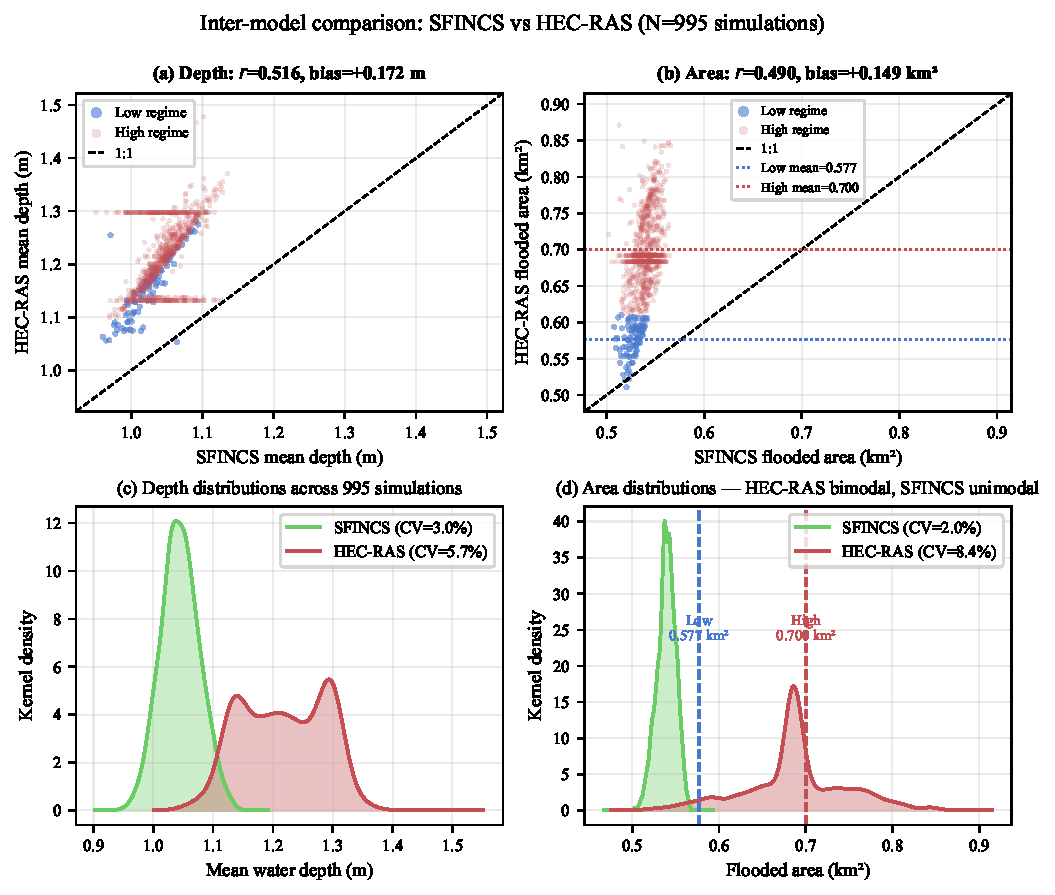
\includegraphics[width=\textwidth]{figures/besaya_fig04_intermodel_comparison.pdf}
  \caption{Comparación de 995 simulaciones emparejadas de SFINCS y HEC-RAS en Los Corrales de Buelna. HEC-RAS produce mayor calado medio y área inundada y presenta una respuesta bimodal que no aparece en SFINCS. Fuente: \parencite{navas2025roughness}.}
  \label{fig:besaya_intermodel}
\end{figure}

La \cref{fig:besaya_intermodel} muestra por qué la automatización masiva no es solo una mejora operativa. La variabilidad entre formulaciones hidráulicas supera la variabilidad atribuible a Manning: HEC-RAS presenta un sesgo medio de $+0{,}172$~m en calado y $+0{,}149$~km\textsuperscript{2} en área respecto a SFINCS, mientras que la correlación entre simulaciones emparejadas es moderada ($r=0{,}52$ para calado y $r=0{,}49$ para área). Una única ejecución no habría permitido identificar esa estructura.

\begin{figure}[htbp]
  \centering
  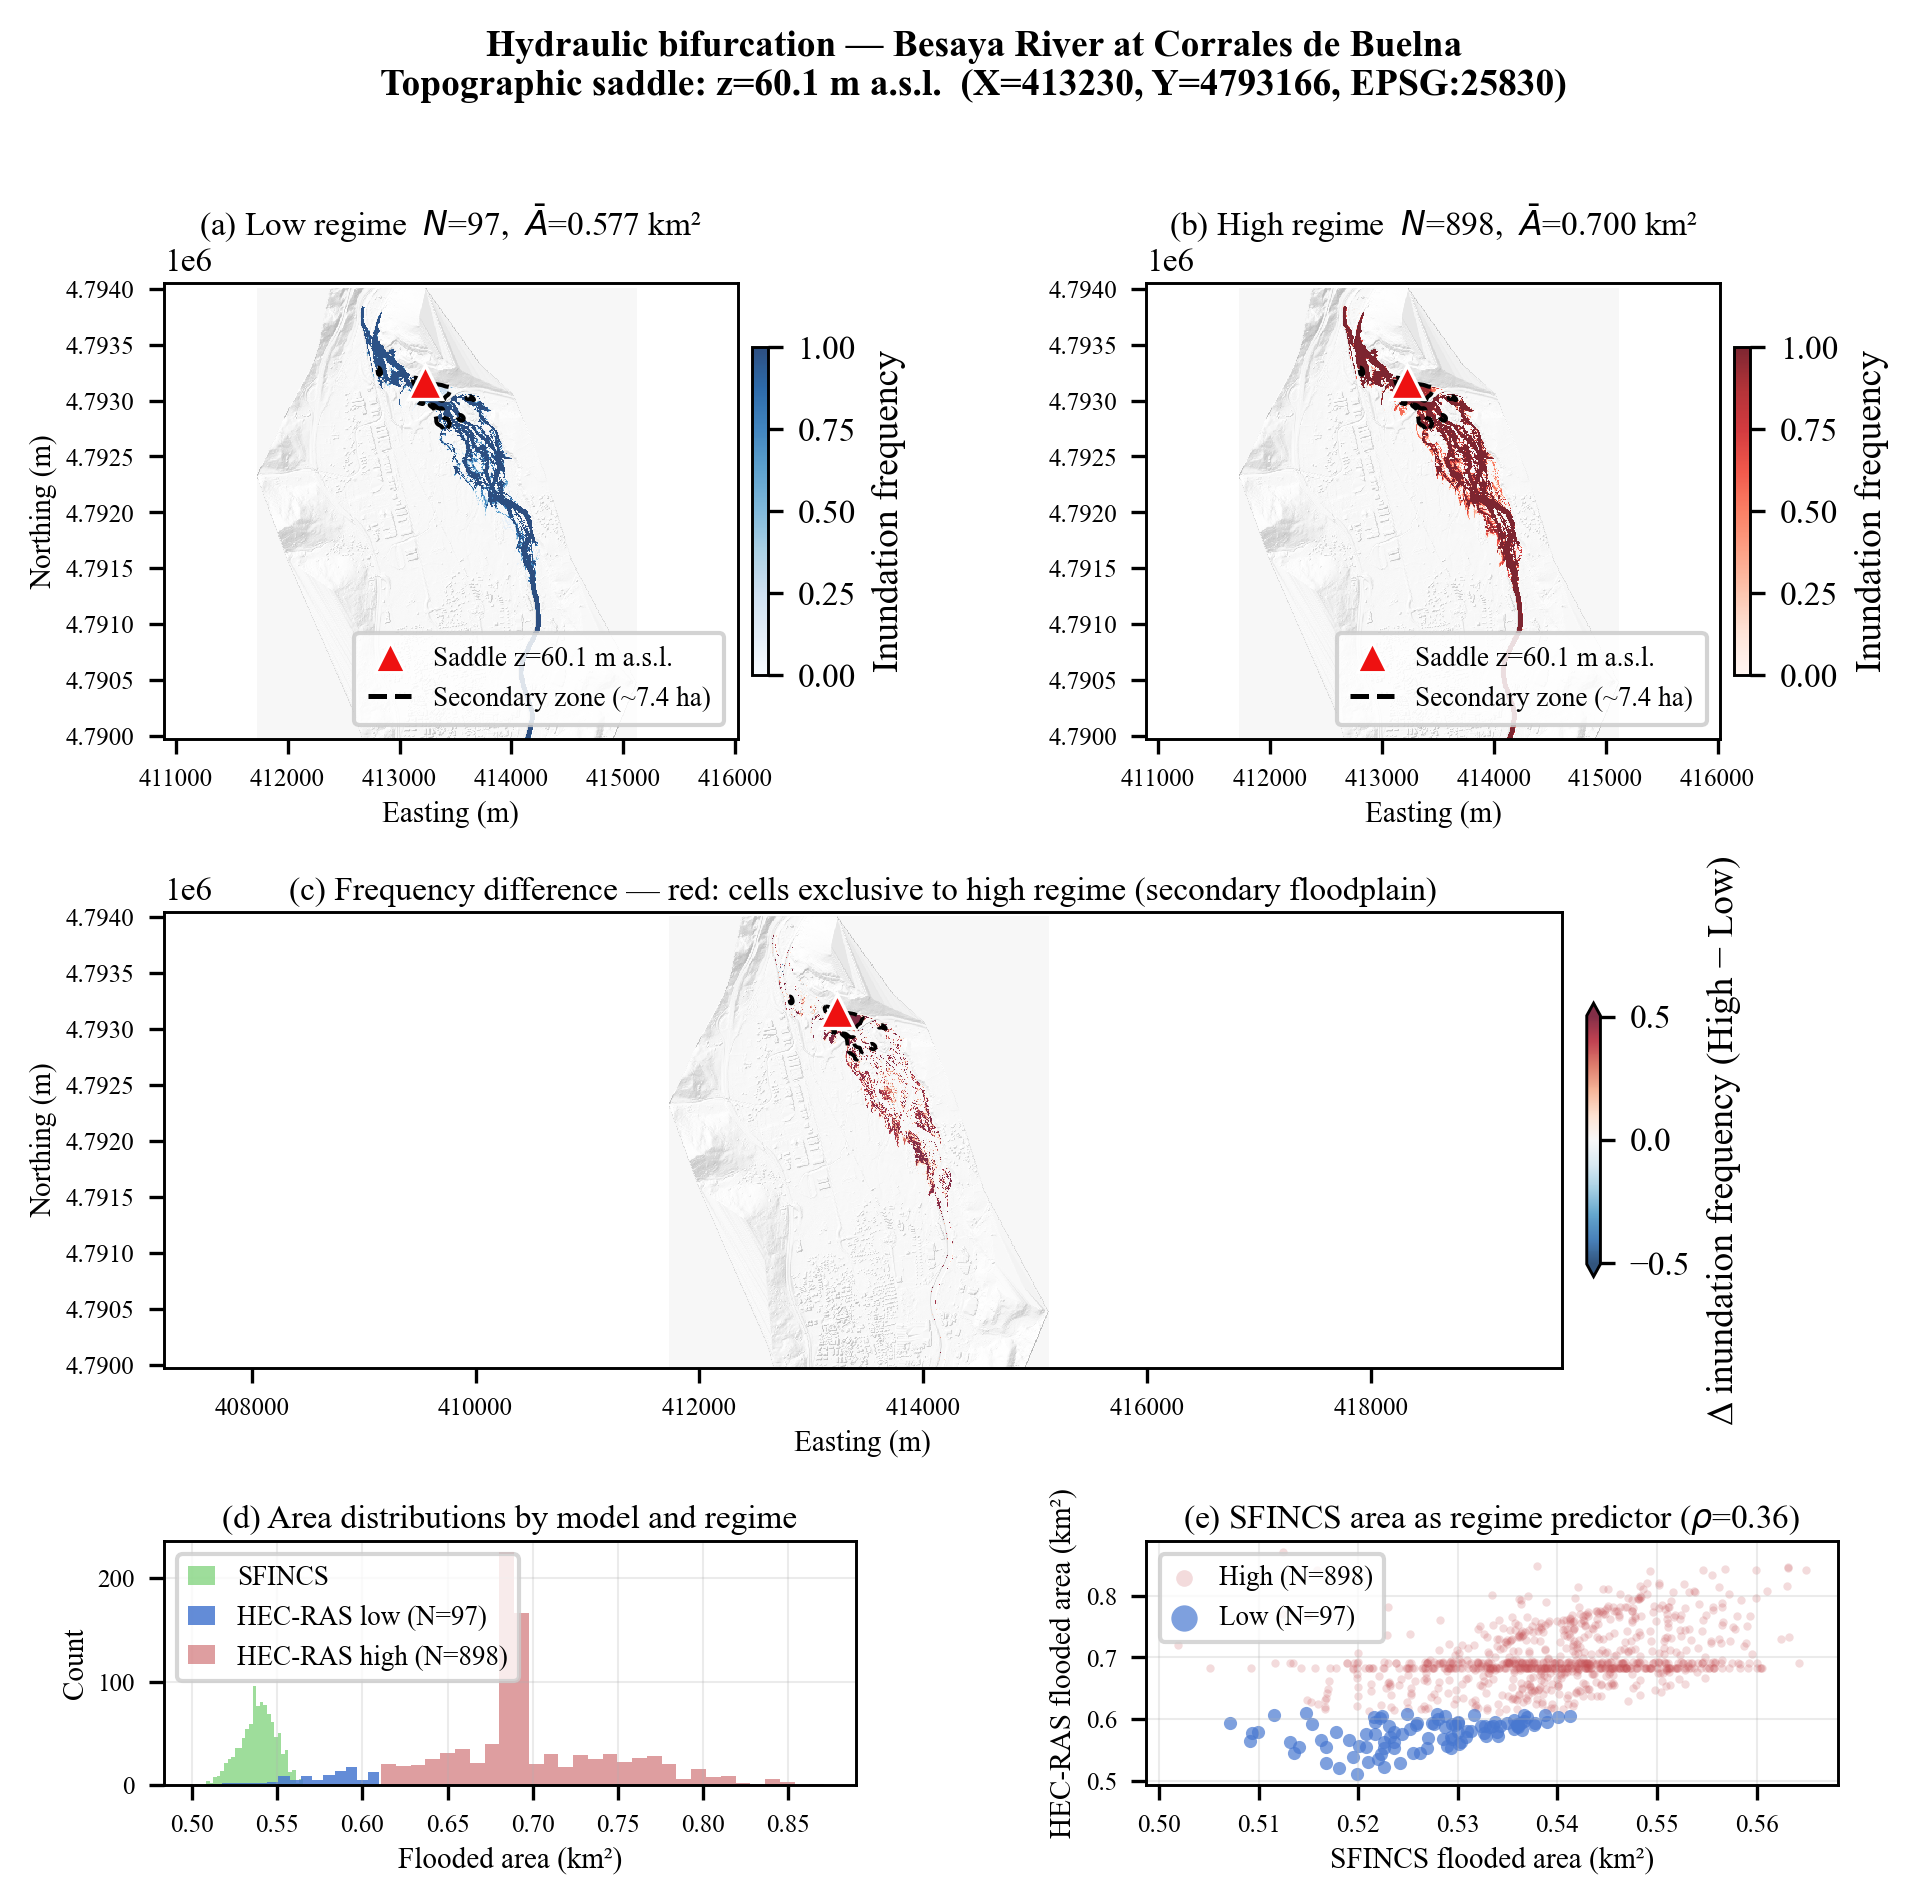
\includegraphics[width=0.95\textwidth]{figures/besaya_fig05_hydraulic_bifurcation.png}
  \caption{Bifurcación hidráulica identificada mediante el ensemble de HEC-RAS. El rebase de un umbral topográfico de aproximadamente 60,1~m activa una llanura secundaria de unas 7,4~ha y separa dos regímenes de área inundada. Fuente: \parencite{navas2025roughness}.}
  \label{fig:besaya_bifurcacion}
\end{figure}

La bifurcación de la \cref{fig:besaya_bifurcacion} evidencia otra aportación de \hydra: conservar salidas espaciales y metadatos de cada ejecución permite pasar de observar una dispersión estadística a explicar su mecanismo físico. Ninguna clase individual de Manning predice el régimen; la transición aparece cuando la dinámica resuelta por HEC-RAS supera un umbral topográfico y conecta una llanura secundaria. Por tanto, el caso valida simultáneamente la cadena estocástica inicial, la ejecución masiva de modelos alternativos y el postprocesado espacial necesario para diagnosticar incertidumbre estructural.

\begin{figure}[htbp]
  \centering
  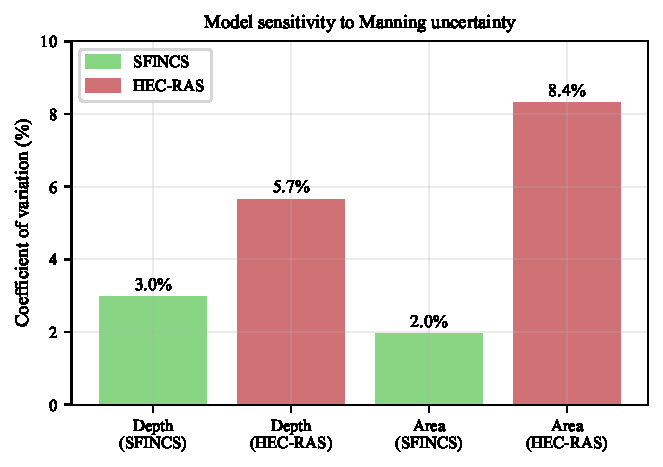
\includegraphics[width=\textwidth]{figures/besaya_fig06_cv_comparison.pdf}
  \caption{Comparación de la variabilidad de calado y área inundada entre SFINCS y HEC-RAS mediante validación cruzada en Los Corrales de Buelna. Los paneles muestran la distribución de los coeficientes de variación para ambas métricas de impacto, desagregados por clase de rugosidad de Manning. La variabilidad intermodelo supera sistemáticamente la variabilidad intramodelo atribuible a Manning. Fuente: \parencite{navas2025roughness}.}
  \label{fig:besaya_cv_comparison}
\end{figure}

\begin{figure}[htbp]
  \centering
  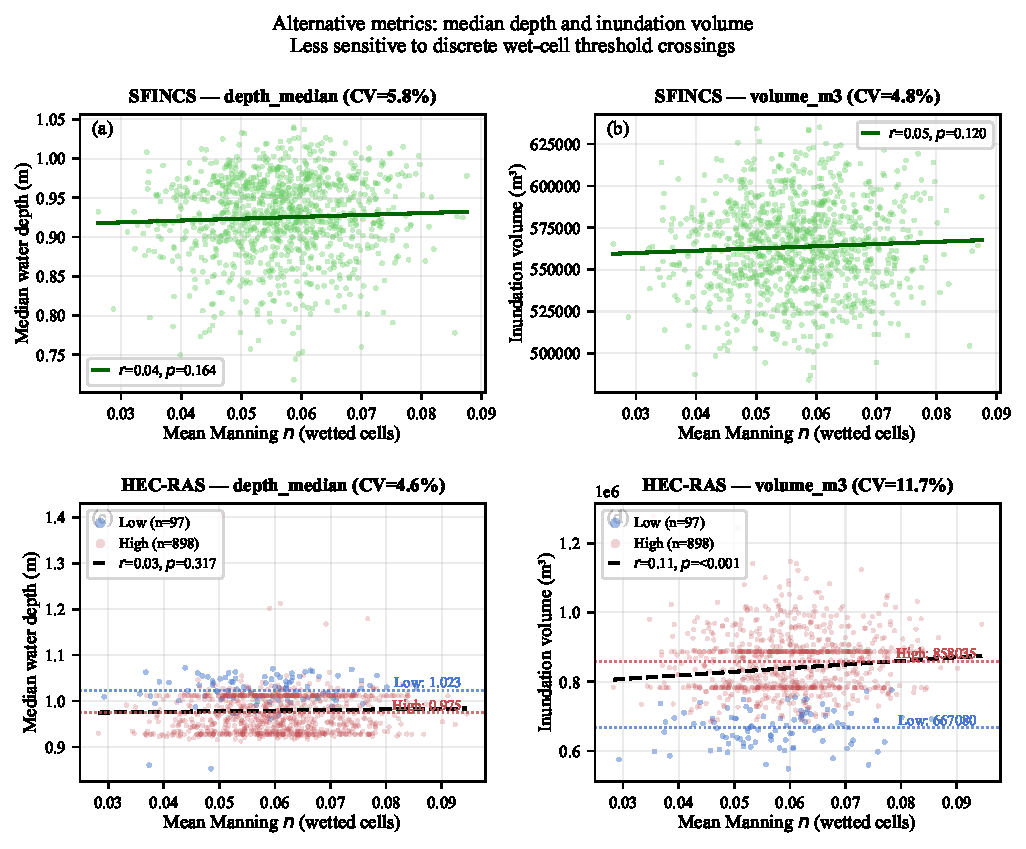
\includegraphics[width=\textwidth]{figures/besaya_fig07_alternative_metrics.pdf}
  \caption{Métricas alternativas de sensibilidad hidráulica en el ensemble de 995 simulaciones emparejadas SFINCS--HEC-RAS. Los paneles muestran índices de concordancia, errores porcentuales y métricas de superposición espacial entre los resultados de ambos modelos. La independencia de las conclusiones respecto a la métrica empleada refuerza la robustez del análisis. Fuente: \parencite{navas2025roughness}.}
  \label{fig:besaya_alternative_metrics}
\end{figure}


\clearpage
\section{Sant Llorenç des Cardassar, Mallorca}
\label{sec:caso_mallorca}

\subsection{Contexto y problema}

El 9 de octubre de 2018 una intensa precipitación convectiva causó el desbordamiento del torrente Ses Planes en la localidad de Sant Llorenç des Cardassar (Mallorca). El episodio acumuló alrededor de 220 litros por metro cuadrado en pocas horas, generando una avenida rápida que provocó pérdidas humanas y daños materiales de gran magnitud. La cuenca del torrente Ses Planes es un ejemplo representativo de régimen hidrológico torrencial mediterráneo: tiempos de concentración inferiores a una hora, pendientes pronunciadas y ausencia de registros de aforo en la sección de interés.

El reto metodológico de este caso es doble. Primero, la generación de escenarios de precipitación plausibles a partir de series pluviométricas cortas y escasas estaciones. Segundo, la obtención de mapas de inundación asociados a períodos de retorno en una cuenca sin calibración de caudal, utilizando como única referencia la mancha de inundación del evento histórico registrada por el servicio Copernicus \parencite{navas2019mallorca}.

\subsection{Metodología aplicada}

La cadena metodológica de este caso arranca desde los pluviómetros horarios del SIAR disponibles en la zona y se complementa con productos satelitales de precipitación. En particular, se utilizó PERSIANN como fuente independiente para contrastar la representatividad espacial de los registros puntuales y para analizar la estructura de la lluvia en el entorno de la cuenca \parencite{ashouri2015persiann}. El notebook interno \texttt{Reconstrucción Precipitación.ipynb} documenta esta fase de trabajo: lectura de SIAR, extracción de celdas PERSIANN, comparación estación-satélite, contraste con TRMM y reconstrucción espacial de la lluvia mediante interpolación geoestadística.

Aunque PERSIANN y TRMM aportaron una referencia espacial externa, no se adoptaron como forzamiento final del modelo hidrológico. La resolución espacial, los sesgos respecto a los pluviómetros horarios y la dificultad para reproducir la estructura local de un episodio convectivo rápido hicieron preferible reconstruir la lluvia con kriging a partir de la red observada. Esta decisión es metodológicamente importante: el caso Mallorca no valida simplemente el uso de datos satelitales, sino la primera formulación de un downscaling híbrido desde precipitación en la línea de investigación, donde los productos remotos sirven para diagnóstico y contraste, mientras que el campo final de lluvia se genera mediante reconstrucción geoestadística controlada por observaciones.

Los eventos de precipitación se detectan y caracterizan mediante cuatro parámetros: precipitación máxima horaria ($P_{max}$), precipitación media del evento ($P_{med}$), duración total y forma del hietograma. Para la clasificación de formas de hietograma se aplica un análisis de componentes principales seguido de K-means, que agrupa los hietogramas históricos en 25 tipos representativos.

A partir de los eventos históricos clasificados se construye un modelo de cópulas gaussianas en \texttt{pyhydra.climate.spatial\_analysis} que preserva la dependencia entre $P_{max}$, $P_{med}$, duración y tipo de hietograma en cada pluviómetro, y la dependencia espacial entre estaciones. Mediante muestreo de la cópula se generan miles de eventos sintéticos que amplían el espacio de escenarios plausibles más allá de los registros históricos disponibles.

De este conjunto se seleccionan los escenarios más representativos mediante el algoritmo de máxima disimilitud en \texttt{pyhydra.climate.hybrid\_downscaling}, reduciendo el número de simulaciones completas a ejecutar. Para cada evento seleccionado se reconstruye el campo de precipitación distribuida sobre la cuenca mediante kriging universal con la elevación como variable de tendencia, produciendo rasters horarios a 25 metros de resolución que se introducen en el módulo hidrológico del modelo Iber. La \cref{fig:mallorca_reconstruccion_lluvia} muestra un ejemplo de reconstrucción horaria del episodio del 9 de octubre de 2018 empleado como referencia para comprobar la coherencia espacio-temporal de los campos de lluvia.

\begin{figure}[htbp]
  \centering
  \begin{tikzpicture}
    \node[inner sep=0] (img) {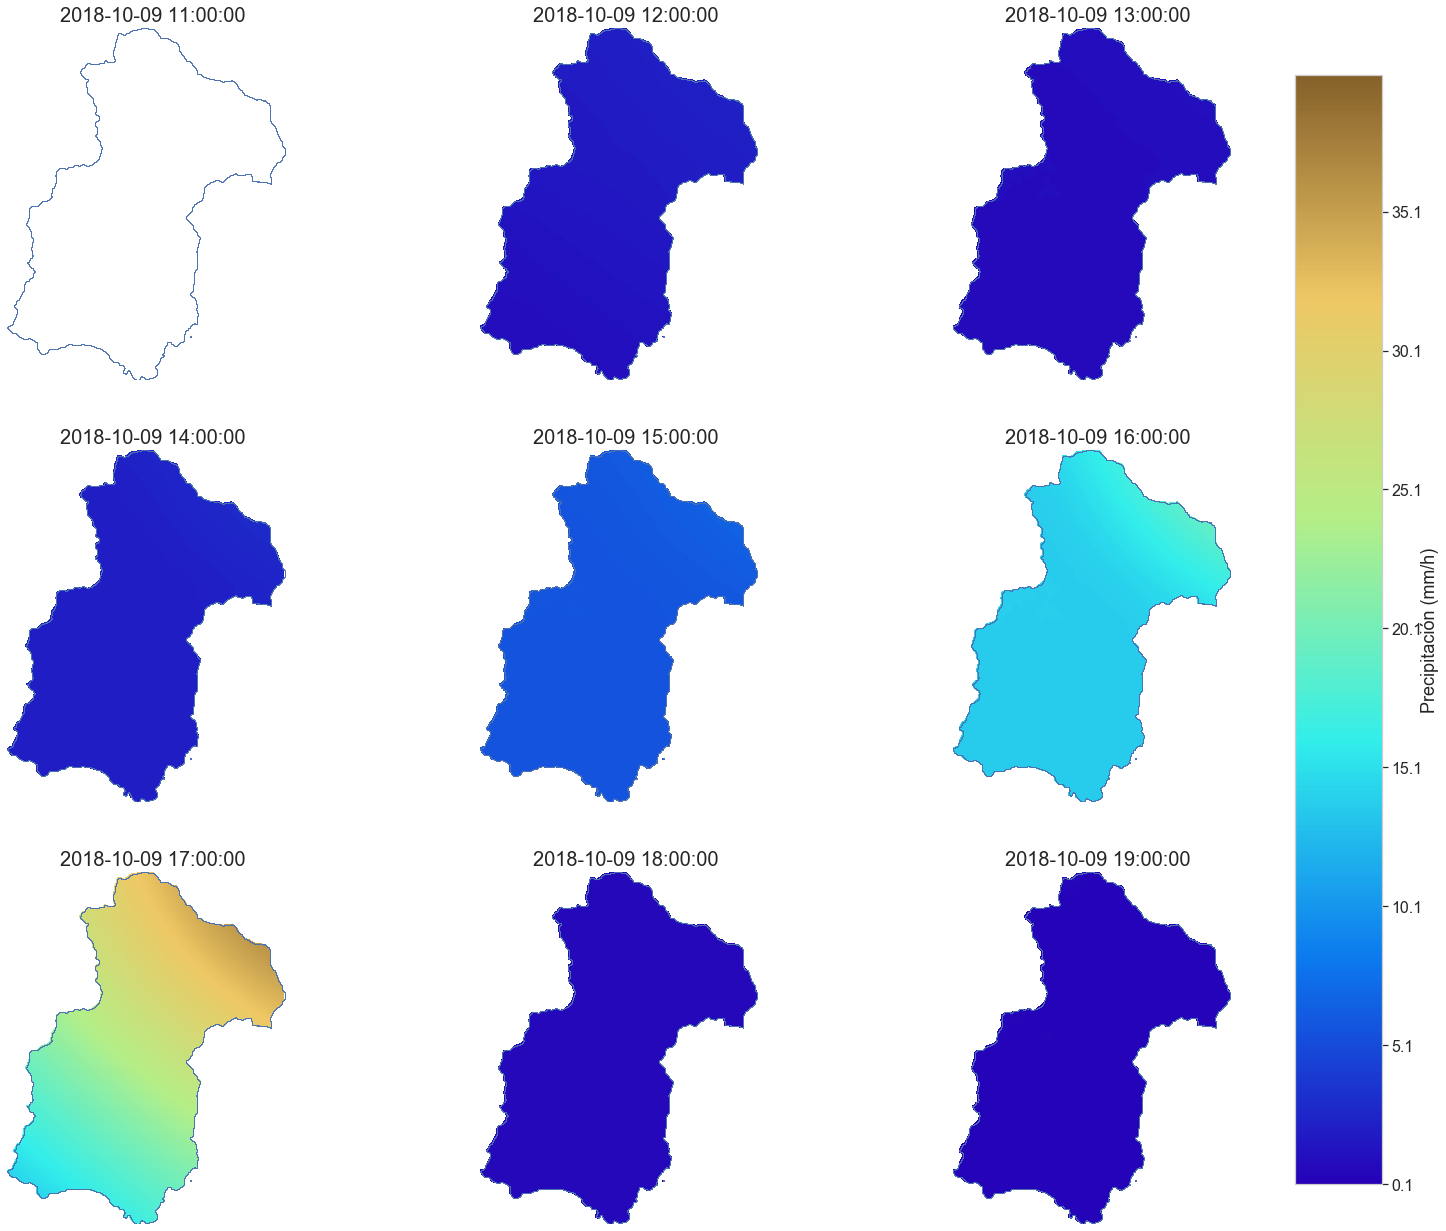
\includegraphics[width=0.94\textwidth]{figures/fig_mallorca_reconstruccion_lluvia.png}};
    \node[font=\small, align=center] at ([yshift=-0.45cm]img.south) {Coordenada horizontal aproximada / longitud};
    \node[font=\small, rotate=90, align=center] at ([xshift=-0.35cm]img.west) {Coordenada vertical aproximada / latitud};
    \node[font=\small, align=center] at ([yshift=0.35cm]img.north) {Campo horario reconstruido mediante kriging};
  \end{tikzpicture}
  \caption{Reconstrucción horaria de la precipitación sobre la cuenca de Sant Llorenç des Cardassar durante el episodio del 9 de octubre de 2018. La figura procede del notebook interno de reconstrucción de precipitación utilizado en el trabajo de Mallorca; se han añadido rótulos editoriales sobre la imagen exportada para mejorar su lectura. Resume la fase de interpolación espacial previa a la simulación hidrológica distribuida.}
  \label{fig:mallorca_reconstruccion_lluvia}
\end{figure}

La simulación hidrológica e hidráulica se realiza en dos fases. La fase hidrológica utiliza la malla de la cuenca completa (MDT 25 m) para transformar la precipitación distribuida en caudales en la sección de entrada a la localidad. La fase hidráulica emplea una malla de mayor resolución (triángulos de 8 m) construida a partir del LiDAR-PNOA del IGN, con los hidrogramas obtenidos de la fase anterior como condición de contorno. La calibración iterativa ajusta los parámetros de infiltración hasta reproducir la mancha de inundación Copernicus del 9 de octubre de 2018, obteniendo calados máximos simulados de hasta 5,85 m en el casco urbano.

Para el conjunto de eventos sintéticos no simulados completamente, los calados y velocidades se reconstruyen mediante k-NN con 6 vecinos, valor óptimo determinado minimizando el error acumulado sobre los 10 últimos eventos simulados de la base de referencia. El resultado final es la distribución empírica de calados en cada celda de la malla hidráulica, con la que se calculan los mapas de período de retorno basados en impacto hidráulico.

\subsection{Resultados y conexión con HYDRA}

El caso Mallorca valida la primera implementación de la cadena de downscaling híbrido basada en precipitación: integración de registros horarios, análisis diagnóstico de precipitación satelital PERSIANN y TRMM, generación de eventos multivariantes con cópulas gaussianas, selección por máxima disimilitud, reconstrucción espacial de campos de lluvia mediante kriging, simulación hidrológica e hidráulica, y reconstrucción de manchas de inundación por k-NN. Es el primer caso en el que la estadística de extremos se aplica sobre variables hidráulicas en lugar de sobre la precipitación forzante, lo que constituye una diferencia metodológica central con los enfoques convencionales.

La comparación entre la mancha simulada para el evento del 9 de octubre de 2018 y la cartografía Copernicus confirma la coherencia del modelo calibrado. La disponibilidad de esa referencia externa independiente es lo que hace de este caso un banco de pruebas válido para la metodología estocástica. Debe precisarse el alcance de esa comparación: la delineación rápida de Copernicus EMS es una referencia de extensión, no de calado, y presenta limitaciones conocidas en zona urbana (sombras de edificación, momento de adquisición posterior al pico de la avenida), por lo que la calibración se evaluó como coherencia de extensión y de niveles máximos en puntos con marcas de avenida documentadas, y no mediante índices de acierto celda a celda. La sistematización de métricas cuantitativas de contraste (índice de acierto crítico sobre la extensión, error de calado en marcas de avenida) sobre este tipo de referencias post-evento forma parte del protocolo de validación descrito en la \cref{sec:validacion_knn} y es directamente aplicable cuando se disponga de levantamientos de campo con calidad suficiente.

\begin{figure}[htbp]
  \centering
  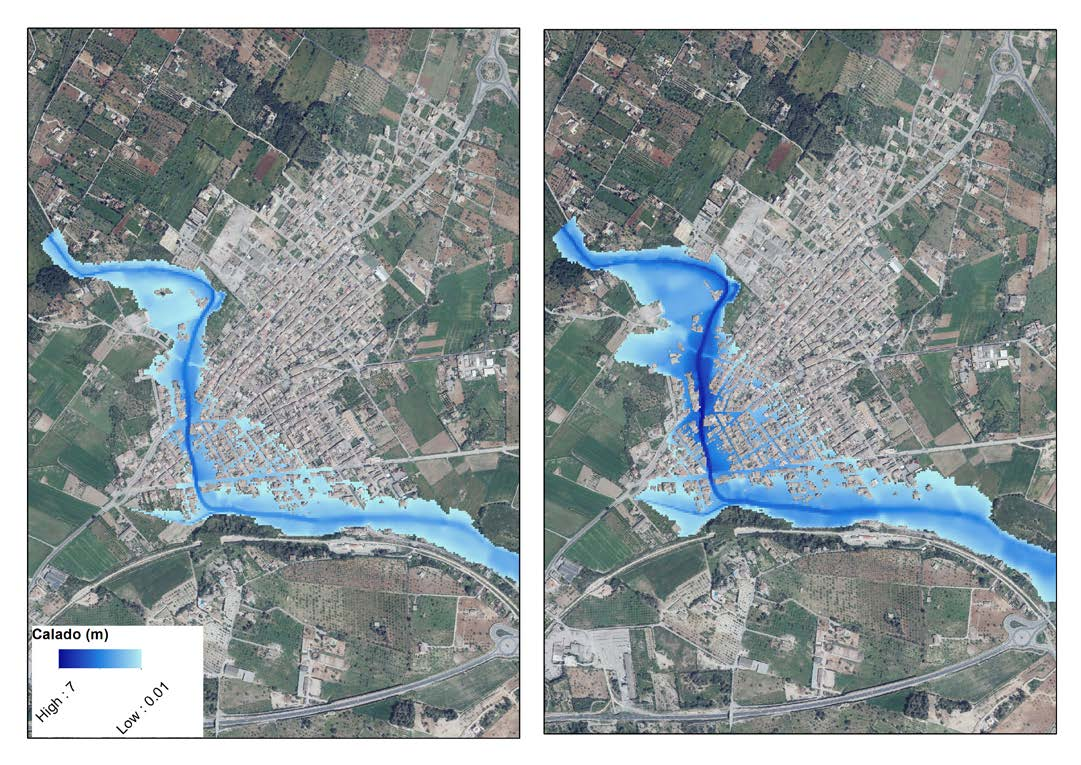
\includegraphics[width=\textwidth]{figures/fig_mallorca_comparativa.png}
  \caption{Comparación de las manchas y calados obtenidos para Sant Llorenç des Cardassar mediante dos formas de caracterizar los eventos de diseño. La aplicación estocástica (derecha) explora una extensión y una distribución de calados diferentes de la obtenida con la metodología habitual (izquierda), ilustrando la importancia de calcular la frecuencia sobre la variable hidráulica final. Fuente: comunicación presentada en las VI Jornadas de Ingeniería del Agua \parencite{navas2019mallorca}.}
  \label{fig:mallorca_calado}
\end{figure}

\clearpage
\section{Calle 30, Madrid}
\label{sec:caso_madrid}

\subsection{Contexto y problema}

La Calle 30 agrupa las infraestructuras soterradas y elevadas de la M-30 en el entorno del río Manzanares en Madrid. Su exposición al riesgo de inundación combina la escorrentía de cuencas externas de mediano tamaño, la precipitación directa y la posibilidad de interacciones con el nivel freático. La complejidad del sistema hidrológico y la importancia de la infraestructura como eje de movilidad metropolitana exigen metodologías capaces de explorar un espacio amplio de escenarios de forzamiento. El caso se presentó inicialmente en las VII Jornadas de Ingeniería del Agua \parencite{deljesus2023calle30} y fue desarrollado posteriormente como artículo \parencite{navas2024calle30,deljesus2024downscaling}.

\begin{figure}[htbp]
  \centering
  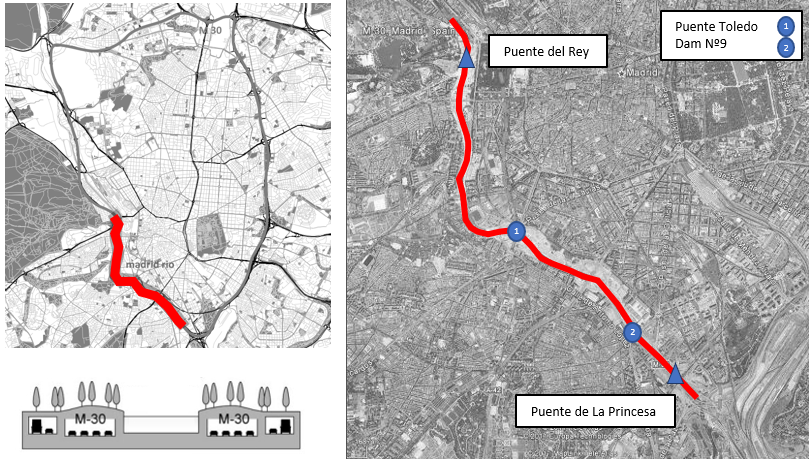
\includegraphics[width=\textwidth]{figures/fig_m30_localizacion}
  \caption{Localización del área de estudio del sistema de infraestructuras Calle 30 -- M-30 en Madrid. El recuadro superior muestra la situación en la Comunidad de Madrid; el inferior delimita el tramo soterrado y las cuencas contribuyentes instrumentadas. Elaboración propia, publicada en \parencite{navas2024calle30}.}
  \label{fig:m30_localizacion}
\end{figure}

\subsection{Metodología aplicada}

La cadena metodológica de Calle 30 es la más completa de los casos aplicados hasta la fecha. Comienza con la descarga y procesamiento de precipitación ERA5 \parencite{hersbach2020era5} y datos pluviométricos de AEMET mediante \texttt{pyhydra.data\_sources.rainfall}. El análisis estadístico de extremos de precipitación multiduracion con GEV en \texttt{pyhydra.climate.time\_series} proporciona las distribuciones de referencia para los forzamientos de diseño.

Los eventos sintéticos se generan mediante cópulas gaussianas multivariantes que modelizan la dependencia entre duraciones y volúmenes de precipitación en las subcuencas contribuyentes. La simulación hidrológica con HEC-HMS produce series de caudales en las secciones de entrada al sistema de drenaje de la M-30. Sobre estas series se aplica la selección de escenarios representativos por máxima disimilitud, seguida de simulación hidráulica completa con HEC-RAS 1D para los escenarios seleccionados. Para el resto, los calados se reconstruyen mediante downscaling híbrido con k-NN \parencite{deljesus2024downscaling}.

El resultado final son mapas de período de retorno basados en calado hidráulico obtenidos con \texttt{pixel\_return\_period} de \texttt{pyhydra.climate.hybrid\_downscaling}, que expresan para cada celda del dominio hidráulico la probabilidad de excedencia anual del calado calculado.

\begin{figure}[!htbp]
\centering
\resizebox{0.98\textwidth}{!}{%
\begin{tikzpicture}[
  font=\scriptsize,
  stat/.style={
    rectangle, rounded corners=5pt,
    minimum width=3.35cm, minimum height=1.15cm,
    text width=3.0cm, align=center,
    draw=tealblock!60!black, fill=tealblock!11,
    line width=0.65pt
  },
  dyn/.style={
    rectangle, rounded corners=5pt,
    minimum width=3.35cm, minimum height=1.15cm,
    text width=3.0cm, align=center,
    draw=orangeblock!70!black, fill=orangeblock!14,
    line width=0.65pt
  },
  hyd/.style={
    rectangle, rounded corners=5pt,
    minimum width=3.35cm, minimum height=1.15cm,
    text width=3.0cm, align=center,
    draw=redstep!60!black, fill=redstep!12,
    line width=0.65pt
  },
  data/.style={
    rectangle, rounded corners=5pt,
    minimum width=3.35cm, minimum height=0.95cm,
    text width=3.0cm, align=center,
    draw=blueblock!65!black, fill=blueblock!10,
    line width=0.6pt
  },
  note/.style={
    rectangle, rounded corners=4pt,
    minimum width=2.9cm, minimum height=0.65cm,
    text width=2.65cm, align=center,
    draw=tg40, fill=tg5,
    line width=0.5pt, font=\scriptsize
  },
  arr/.style={-Stealth, line width=0.8pt, color=tg55}
]
\node[data] (rain) at (0,3.2) {\textbf{Precipitación}\\ERA5 + pluviómetros};
\node[stat] (sep) at (3.95,3.2) {\textbf{Eventos de lluvia}\\duración, volumen, intensidad};
\node[stat] (cop) at (7.9,3.2) {\textbf{Cópulas multivariantes}\\dependencia espacial y temporal};
\node[stat] (synt) at (11.85,3.2) {\textbf{Eventos sintéticos}\\precipitación en subcuencas};


\node[stat] (selecthms) at (11.85,1.35) {\textbf{Selección inicial}\\escenarios para HEC-HMS};
\node[dyn] (hms) at (7.9,1.35) {\textbf{Simulación hidrológica}\\HEC-HMS};
\node[stat] (maxdiss) at (3.95,1.35) {\textbf{Selección hidráulica}\\MaxDiss sobre hidrogramas};

\node[data] (terrain) at (0,-0.75) {\textbf{Modelo urbano}\\MDT, drenaje, geometría};
\node[hyd] (ras) at (3.95,-0.75) {\textbf{Simulación hidráulica}\\HEC-RAS 1D};
\node[stat] (knn) at (7.9,-0.75) {\textbf{Reconstrucción k-NN}\\mapas no simulados};
\node[hyd] (rp) at (11.85,-0.75) {\textbf{Períodos de retorno}\\calado por pixel};

\draw[arr] (rain) -- (sep);
\draw[arr] (sep) -- (cop);
\draw[arr] (cop) -- (synt);
\draw[arr] (synt.south) -- (selecthms.north);
\draw[arr] (selecthms.west) -- (hms.east);
\draw[arr] (hms.west) -- (maxdiss.east);
\coordinate (m30MaxOut) at (3.95,0.35);
\draw[arr] (maxdiss.south) -- (m30MaxOut) -- (ras.north);
\draw[arr] (terrain) -- (ras);
\draw[arr] (ras) -- (knn);
\draw[arr] (knn) -- (rp);
\end{tikzpicture}
}
\caption{Esquema metodológico del caso Calle 30--M-30 Madrid \parencite{navas2024calle30,deljesus2024downscaling}. A diferencia del Besaya, el flujo parte de precipitación multisitio: los eventos de lluvia se generan con cópulas, se transforman en caudales con HEC-HMS, se selecciona un subconjunto hidráulicamente representativo con MaxDiss y se simula con HEC-RAS 1D. La reconstrucción k-NN de los resultados no simulados constituye el downscaling híbrido.}
\label{fig:m30_esquema_precipitacion}
\end{figure}

\subsection{Resultados y conexión con HYDRA}

Los resultados del estudio \parencite{navas2024calle30} son mapas de calado asociados a distintos períodos de retorno en el entorno de la M-30 semienterrada. La comparación con evaluaciones previas disponibles para la misma área confirma la coherencia de los resultados y cuantifica la diferencia entre el período de retorno del forzamiento meteorológico y el del impacto hidráulico, que en sistemas urbanos con efectos de atenuación o concentración puede ser significativa.

El caso Calle 30 es la validación de referencia de la Tarea 2 del plan de investigación: la combinación de generación estocástica, máxima disimilitud, simulación hidráulica y reconstrucción k-NN para obtener períodos de retorno basados en variables de impacto. Es el caso sobre el que se ha definido la interfaz entre todos los módulos de \hydra.

\paragraph{Justificación de las herramientas.}
En Calle 30, el uso de \hydra se justifica por la combinación de tres fuentes de complejidad sintetizadas en la \cref{fig:m30_esquema_precipitacion}. Primero, varios pluviómetros y subcuencas producen forzamientos espacialmente dependientes, por lo que las cópulas evitan generar escenarios incompatibles entre puntos. Segundo, cada escenario exige encadenar HEC-HMS y HEC-RAS 1D, de modo que la automatización de entradas y salidas es necesaria para mantener la trazabilidad. Tercero, el coste de HEC-RAS impide simular exhaustivamente el conjunto sintético, lo que hace necesaria la selección MaxDiss y la reconstrucción k-NN. La utilidad de cada módulo queda así vinculada a una necesidad verificable del caso, no solo a la disponibilidad de la herramienta.

\clearpage
\section{Valencia: análisis del episodio DANA de octubre 2024}
\label{sec:caso_valencia}

\subsection{Contexto y problema}

El 29 de octubre de 2024 una depresión aislada en niveles altos (DANA) generó precipitaciones extremas en la Comunidad Valenciana. La estación 8337X en Turís registró 710,8 mm en 24 horas, estableciendo un récord nacional. La estación V103 en Carlet registró 265,1 mm en el mismo período. Ambas estaciones están separadas aproximadamente 21,7 km. El evento causó más de 220 víctimas y daños materiales de magnitud excepcional en el área metropolitana de Valencia.

El problema estadístico que plantea el episodio es la estimación del período de retorno de precipitación extrema de corta duración en una región con alta variabilidad interanual, series pluviométricas de longitud limitada y registros históricos que no habían incluido jamás un evento de esta magnitud. En estas condiciones, los métodos clásicos de estimación muestran una sensibilidad extrema a la inclusión o exclusión del evento en la serie, con estimaciones de período de retorno que varían en órdenes de magnitud dependiendo del enfoque utilizado \parencite{deljesus2025jia}.

\subsection{Metodología aplicada}

El estudio aplica y compara tres métodos de ajuste de la distribución GEV sobre series de máximos anuales de precipitación diaria acumulada en dos niveles de análisis: individual por estación y regional de frecuencia.

El análisis individual se centra en las estaciones 8337X (Turís) y V103 (Carlet). Se ajusta la distribución GEV mediante máxima verosimilitud (MLE), L-momentos y estimación bayesiana con priors débiles mediante MCMC hamiltoniano (4 cadenas, 1000 muestras) con PyMC, siguiendo la estructura del módulo \texttt{pyhydra.climate.time\_series}. Para cada método se comparan dos escenarios: con y sin la inclusión del evento de 2024 en la serie.

El análisis regional de frecuencia se aplica a dos escalas. El RFA local utiliza un grupo de 9 estaciones ubicadas en el entorno de Turís y Carlet, seleccionadas por proximidad espacial y coherencia pluviométrica. El RFA global utiliza una red ampliada de estaciones distribuidas por la Comunidad Valenciana. En ambos casos se emplea el procedimiento de Hosking y Wallis \parencite{hosking1997rfa}: estandarización de series (Z-score por estación), construcción de la muestra regional (máximo anual entre estaciones estandarizadas), y ajuste GEV a la serie regional mediante los tres métodos. La transferencia a escala local se realiza mediante la transformación inversa $z_{T,i} = y_T \cdot s_i + \bar{x}_i$, donde $y_T$ es el cuantil regional adimensional para el período de retorno $T$, y $s_i$ y $\bar{x}_i$ son la desviación típica y la media empíricas de la estación de interés. El conjunto de datos empleado comprende 224 estaciones (30 AEMET, 41 SIAR, 153 AVAMET).

\subsection{Resultados}

Los resultados del análisis individual muestran una sensibilidad extrema de los métodos clásicos a la inclusión del evento. Sin incluir la DANA, el método bayesiano estima para Turís un nivel de precipitación de 260 mm para un período de retorno de 100 años y 417,6 mm para 500 años. Al incluir el evento, las mismas estimaciones ascienden a 952 mm y 3004 mm respectivamente (Tabla~\ref{tab:results_valencia_individual}). Para los L-momentos la variación es menos pronunciada pero mantiene la misma tendencia.

\begin{table}[htbp]
  \centering
  \caption{Niveles de precipitación estimados (mm) para distintos períodos de retorno en Turís y Carlet. Análisis individual. El valor bayesiano se expresa en mm; MLE y L-momentos como porcentaje de cambio respecto al bayesiano.}
  \label{tab:results_valencia_individual}
  \resizebox{\textwidth}{!}{%
  \begin{tabular}{llrrrrrrr}
    \toprule
    & & \multicolumn{3}{c}{Sin considerar DANA} & \multicolumn{3}{c}{Considerando DANA} \\
    \cmidrule(lr){3-5}\cmidrule(lr){6-8}
    Estación & T & Bayes (mm) & MLE (\%) & L-mom (\%) & Bayes (mm) & MLE (\%) & L-mom (\%) \\
    \midrule
    Turís & 10  & 126,0 & -5,5 & -5,1 & 195,2 & -4,9 & -15,3 \\
    (8337X) & 100 & 260,2 & -12,7 & -16,2 & 952,0 & -13,7 & -20,6 \\
           & 500 & 417,6 & -18,6 & -25,3 & 3004,1 & -21,0 & -24,0 \\
    \midrule
    Carlet & 10  & 125,5 & -3,7 & -2,6 & 146,3 & -3,9 & -3,3 \\
    (V103) & 100 & 202,8 & -8,7 & -7,0 & 293,0 & -8,3 & -1,7 \\
           & 500 & 262,2 & -11,9 & -10,1 & 450,5 & -11,9 & -0,3 \\
    \bottomrule
  \end{tabular}}
\end{table}

El período de retorno estimado para los valores observados el 29 de octubre de 2024 (710,8 mm en Turís, 265,1 mm en Carlet) es especialmente revelador. Sin incluir el evento en la serie, los métodos clásicos estiman períodos de retorno superiores a 11.000 años en Turís (MLE) y de más de 31.000 años (L-momentos), mientras que el método bayesiano estima 3.069 años. Al incluir el evento, las estimaciones descienden bruscamente a valores coherentes: entre 66 y 91 años en Turís y entre 70 y 95 años en Carlet (Tabla~\ref{tab:returns_valencia}).

\begin{table}[htbp]
  \centering
  \caption{Períodos de retorno estimados (años) para los valores observados el 29 de octubre de 2024. Análisis individual.}
  \label{tab:returns_valencia}
  \resizebox{0.85\textwidth}{!}{%
  \begin{tabular}{lrrrrrrr}
    \toprule
    & \multicolumn{3}{c}{Sin considerar DANA} & \multicolumn{3}{c}{Considerando DANA} \\
    \cmidrule(lr){2-4}\cmidrule(lr){5-7}
    Estación & Bayes & MLE & L-mom & Bayes & MLE & L-mom \\
    \midrule
    Turís (710,8 mm)  & 3069 & 11453 & 31345 & 66 & 80 & 91 \\
    Carlet (265,1 mm) & 536  & 1616  & 1329  & 70 & 95 & 75 \\
    \bottomrule
  \end{tabular}}
\end{table}

El análisis RFA local (9 estaciones próximas) produce estimaciones más estables que el análisis individual: el período de retorno del evento en Turís, sin incluir la DANA, se estima entre 581.741 y 7.549.328 años (valores sin sentido práctico), mientras que al incluirlo desciende a 34-41 años. El RFA global tiende a suavizar los efectos del evento extremo, produciendo períodos de retorno de 10-19 años en Turís con la DANA incluida.

\begin{figure}[htbp]
  \centering
  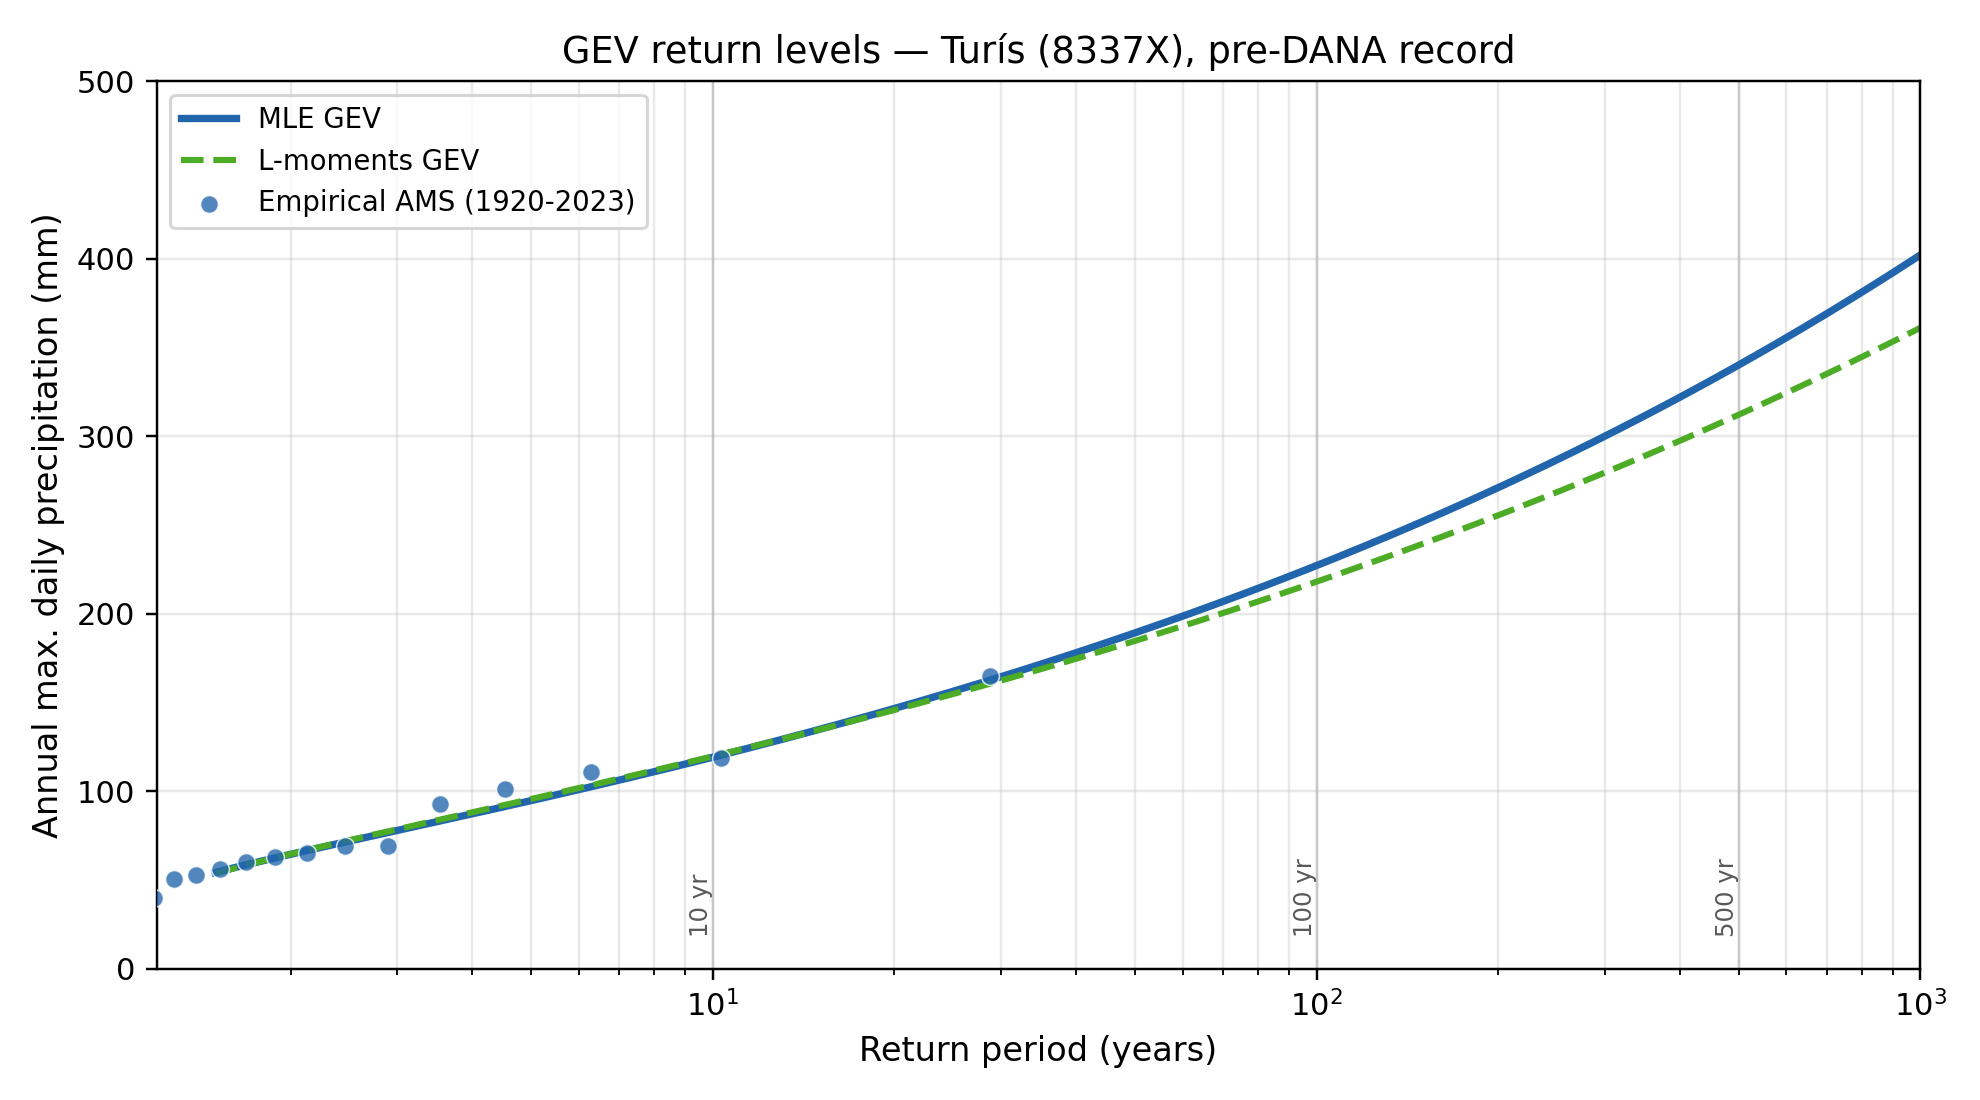
\includegraphics[width=\linewidth]{figures/fig_valencia_curvas_retorno_pre_dana_notebook.png}
  \caption[Curvas de nivel de retorno GEV pre-DANA en Turís]{Curvas de nivel de retorno GEV para la estación 8337X (Turís), obtenidas con la serie de máximos anuales previa al episodio de 2024 en el notebook \texttt{pilot\_cases/valencia\_dana/02\_extreme\_value\_analysis.ipynb}. La curva azul corresponde al ajuste por máxima verosimilitud y la curva verde al ajuste por L-momentos; los puntos representan las posiciones empíricas de los máximos anuales disponibles hasta 2023. Salida computada del notebook del caso Valencia.}
  \label{fig:valencia_curvas_retorno}
\end{figure}

\begin{figure}[p]
  \centering
  \begin{subfigure}{0.94\textwidth}
    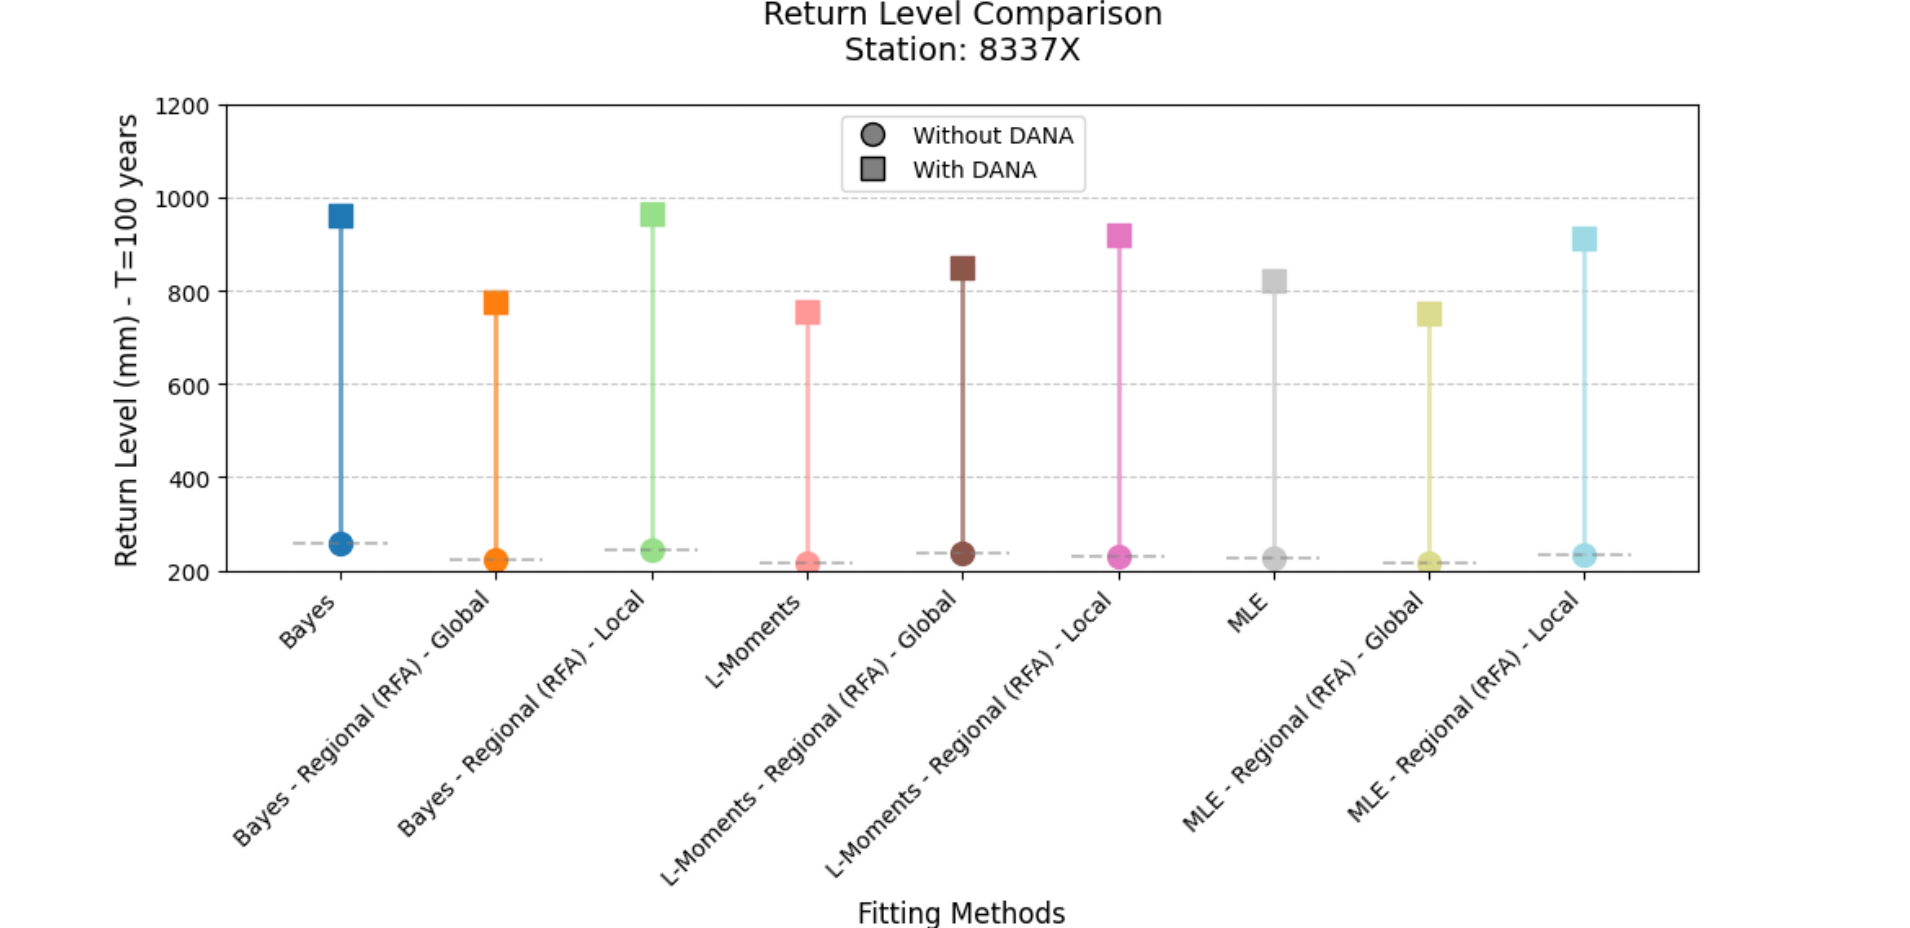
\includegraphics[width=\textwidth]{figures/fig_valencia_return_levels_8337X_clean.png}
    \caption{Turís (8337X).}
    \label{fig:valencia_rl_turis}
  \end{subfigure}
  \vspace{0.8em}
  \begin{subfigure}{0.94\textwidth}
    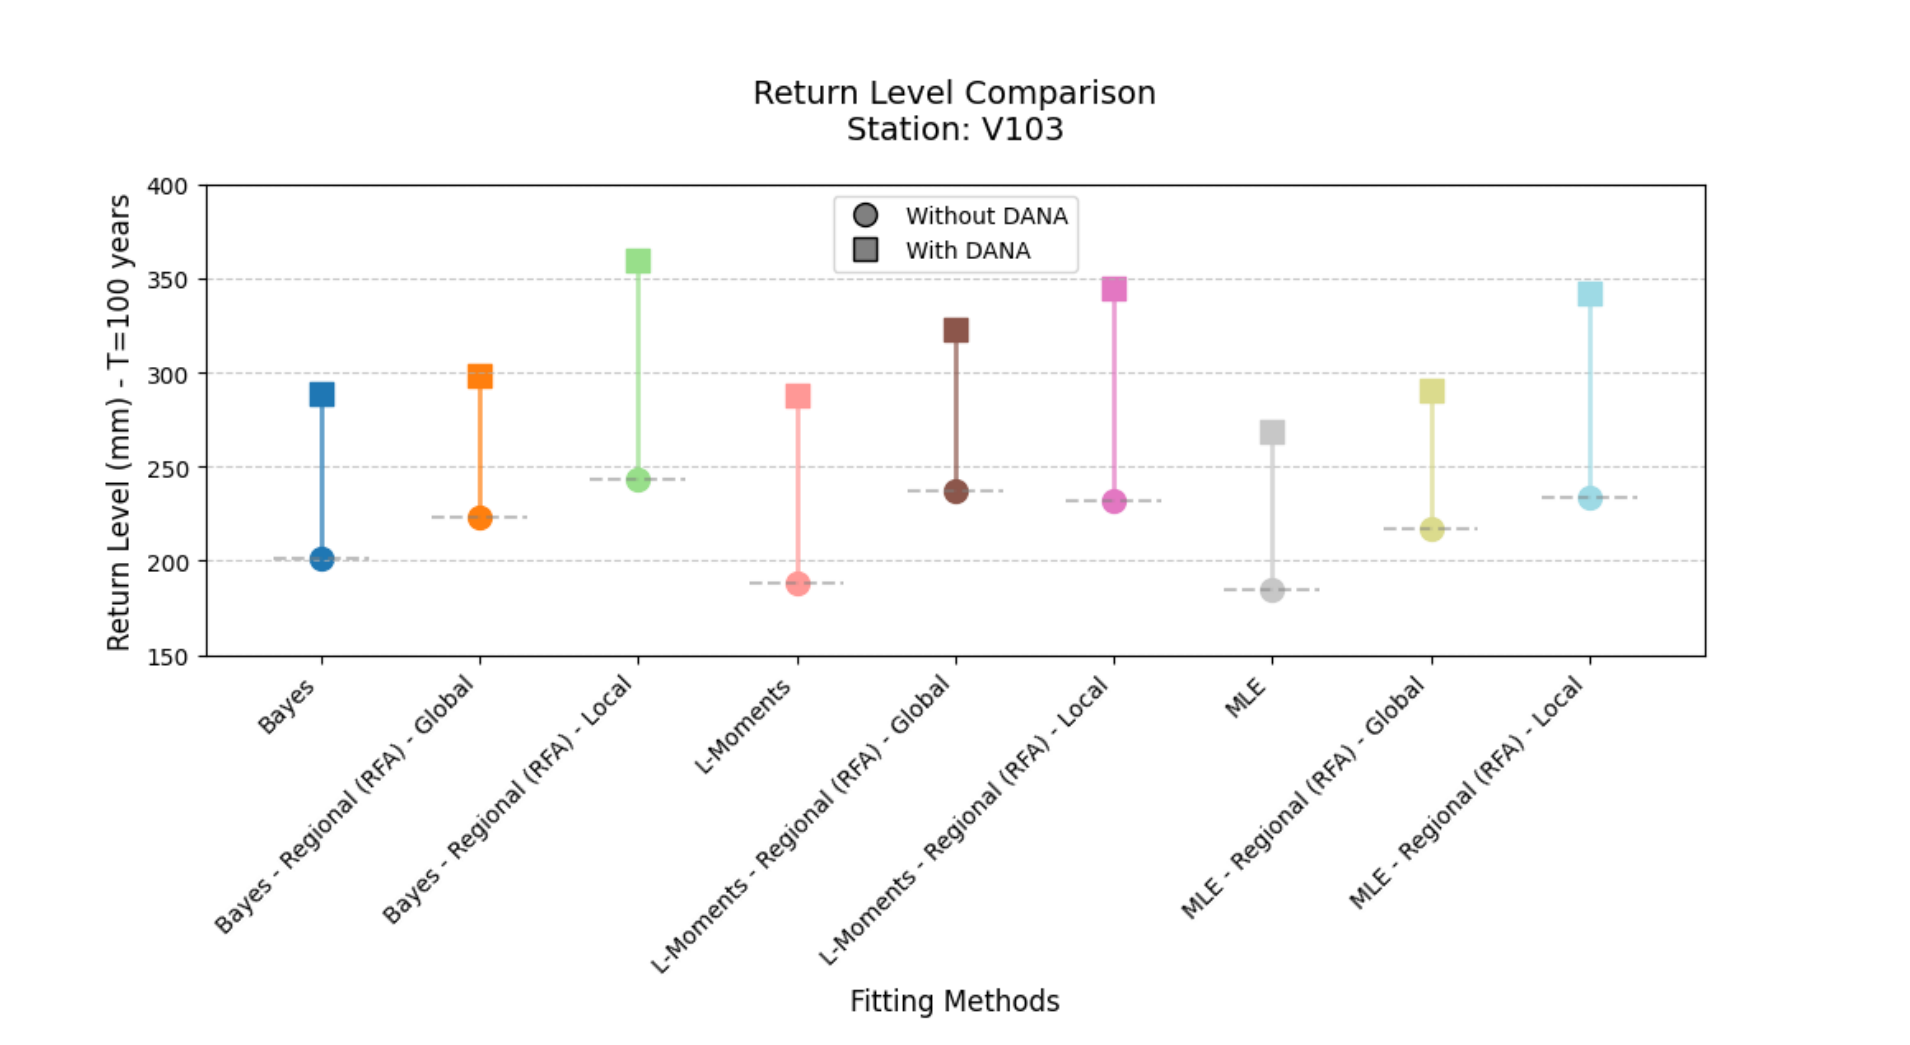
\includegraphics[width=\textwidth]{figures/fig_valencia_return_levels_V103_clean.png}
    \caption{Carlet (V103).}
    \label{fig:valencia_rl_carlet}
  \end{subfigure}
  \caption{Comparación de niveles de retorno para $T=100$ años en las estaciones de Turís y Carlet, con y sin inclusión del episodio DANA del 29 de octubre de 2024. La figura procede del análisis reproducible del caso Valencia \parencite{navas2025valenciaIA} y se incorpora como evidencia de contraste metodológico.}
  \label{fig:valencia_return_levels}
\end{figure}

\subsection{Conexión con HYDRA}

El caso Valencia valida los módulos de análisis de extremos de \path{pyhydra.climate.time_series} en un escenario de urgencia post-evento. La comparación entre MLE, L-momentos y estimación bayesiana sobre las mismas series, con y sin inclusión del evento, ilustra con datos reales por qué la disponibilidad de múltiples métodos de estimación es esencial para comunicar adecuadamente la incertidumbre. La implementación del RFA en \path{pyhydra.climate.spatial_analysis} permite reproducir el flujo completo, desde la descarga de datos de las redes AEMET, SIAR y AVAMET hasta la estimación de cuantiles regionales con intervalos credibles.

La conclusión principal del estudio \parencite{navas2025valenciaIA} es que el método bayesiano proporciona estimaciones más estables y coherentes entre escenarios que los métodos clásicos, al representar explícitamente la incertidumbre en los parámetros y en los cuantiles de retorno. Esta conclusión refuerza la decisión de incluir \texttt{fit\_gev\_mcmc} como alternativa preferente en \hydra para análisis en regiones con alta variabilidad o series cortas.

\clearpage
\section{Lago Tanganica: niveles de diseño bajo cambio climático}
\label{sec:caso_tanganika}

\subsection{Contexto y problema}

El Lago Tanganica, en la región de los Grandes Lagos de África, es una masa de agua compartida por Burundi, República Democrática del Congo, Tanzania y Zambia, con una cuenca de más de 230.000 km\textsuperscript{2}. La variabilidad creciente de sus niveles, atribuida al cambio climático, plantea riesgos directos sobre infraestructuras costeras como el puerto de Kalundu (Burundi). El diseño de la nueva infraestructura portuaria requiere definir cotas de nivel para distintos períodos de retorno bajo escenarios futuros de emisión, en un contexto donde los registros instrumentales continuos son muy limitados \parencite{navas2025tanganika}.

Este caso ilustra cómo la metodología de \hydra puede extenderse a sistemas lacustres en regiones con escasa instrumentación, combinando datos de teledetección, reanálisis climático y proyecciones CMIP6.

\subsection{Metodología aplicada}

La cadena metodológica se estructura en cinco etapas secuenciales. La primera estima los caudales mensuales de entrada al lago a partir de variables climáticas del reanálisis ERA5 \parencite{hersbach2020era5} mediante un modelo de regresión multivariante. Las variables predictoras (precipitación, temperatura máxima y mínima, radiación solar, velocidad del viento) se normalizan por celda y se someten a análisis de componentes principales para eliminar la multicolinealidad. Se comparan varios algoritmos de aprendizaje automático (regresión lineal, Elastic Net, SVR, árboles de decisión, Gradient Boosting, AdaBoost). El modelo seleccionado, AdaBoost Regressor, obtiene un coeficiente de determinación $R^2 > 0{,}85$ en validación cruzada y $R^2 = 0{,}96$ sobre el conjunto completo, con RMSE inferior al 10\% del rango observado.

La segunda etapa construye una función empírica continua caudal-nivel $N(Q)$ mediante K-means (3 clusters: caudales bajos, medios y altos) y ajuste de funciones polinómicas de segundo grado para los dos primeros grupos y una función potencial para el tercero. Esta función transforma las series de caudal simuladas en series de nivel del lago, incorporando la no linealidad de la respuesta hidrológica.

La tercera etapa incorpora la señal del cambio climático mediante downscaling estadístico de 19 modelos CMIP6 bajo los escenarios SSP2-4.5 y SSP5-8.5. Se emplea el método delta mes a mes disponible en \texttt{pyhydra.climate.bias\_correction}, que conserva la variabilidad espacial y temporal de las observaciones ERA5 mientras incorpora la anomalía climática proyectada. Los datos CMIP6 se descargan vía CDS con \texttt{pyhydra.data\_sources.climate\_change}.

La cuarta etapa genera series sintéticas de nivel mediante remuestreo bootstrap de los residuos del modelo caudal-nivel por tramo. Para cada mes de cada realización se añade a $\tilde{N}(Q_t)$ un residuo aleatorio extraído de la distribución empírica del tramo correspondiente. Este proceso se repite 1.000-2.000 veces por combinación de modelo y escenario, generando un total de aproximadamente 20.000 años simulados que cubren explícitamente la incertidumbre de la función empírica $N(Q)$.

La quinta etapa estima los niveles extremos de forma no paramétrica a partir de los percentiles empíricos de los máximos anuales del conjunto sintético. Las variaciones proyectadas $\Delta Nivel(T, t) = N_{fut}(T, t) - N_{hist}(T)$ se aplican sobre los niveles históricos obtenidos con GEV ajustada a la serie observada de altimetría satelital (Hydroweb, 1992-2023), generando proyecciones absolutas de nivel que combinan la robustez empírica del registro histórico con la señal climática proyectada.

\subsection{Resultados}

Los niveles históricos extremos estimados a partir de distribuciones teóricas (GEV, Weibull) arrojan valores de 771,55-771,76 m para un período de retorno de 100 años. El enfoque bootstrap produce niveles sistemáticamente menores para los mismos períodos de retorno (770,19 m para T100), diferencia atribuible al efecto suavizador del remuestreo sobre los valores extremos atípicos.

Las proyecciones bajo cambio climático muestran incrementos sistemáticos de los niveles máximos a lo largo del siglo XXI en ambos escenarios. El mayor incremento proyectado se alcanza en el período 2041-2060, donde los niveles máximos asociados a períodos de retorno cortos (T5-T10) aumentan más de 0,9 m respecto al histórico. Hacia el final del siglo (2081-2100), los incrementos se estabilizan por debajo de 0,6 m para los períodos de retorno largos (T100-T500), efecto atribuido a la expansión superficial del lago que amortigua los cambios de nivel a medida que el volumen adicional se distribuye sobre una mayor área. Las diferencias entre SSP2-4.5 y SSP5-8.5 son marcadas en las primeras décadas y convergen hacia el final del siglo.

\begin{figure}[htbp]
  \centering
  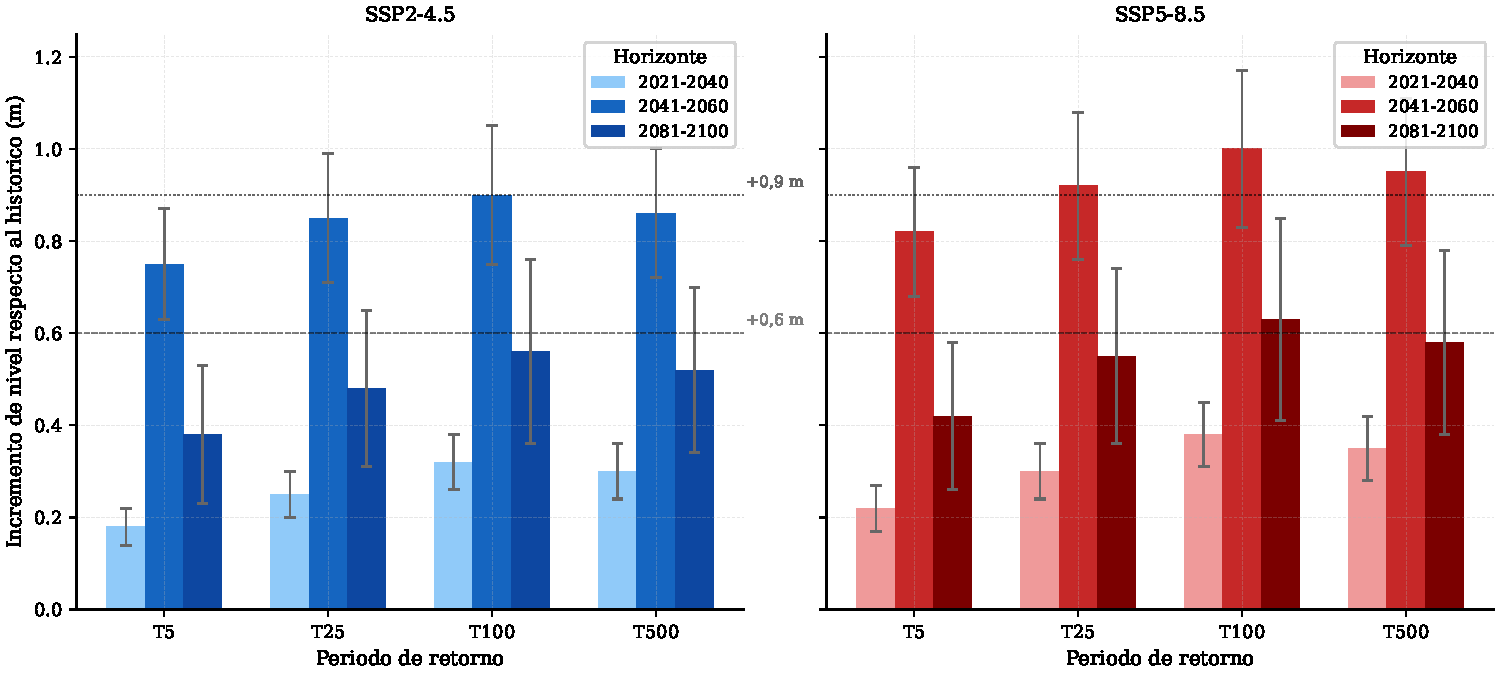
\includegraphics[width=\linewidth]{figures/fig_tanganika_proyecciones}
  \caption{Evolución del caudal mensual proyectado de entrada al Lago Tanganica (m$^3$/s), estimado con el modelo AdaBoost bajo condiciones históricas (gris) y bajo los escenarios de cambio climático SSP2-4.5 (azul) y SSP5-8.5 (rojo), con bandas de incertidumbre intermodelo. La línea vertical marca el inicio del período de proyección (2022). Ambos escenarios proyectan un incremento sostenido del caudal medio hacia finales del siglo XXI, con mayor variabilidad interanual. Figura reproducida de \parencite{navas2025tanganicaIA}.}
  \label{fig:tanganika_proyecciones}
\end{figure}

\begin{figure}[htbp]
  \centering
  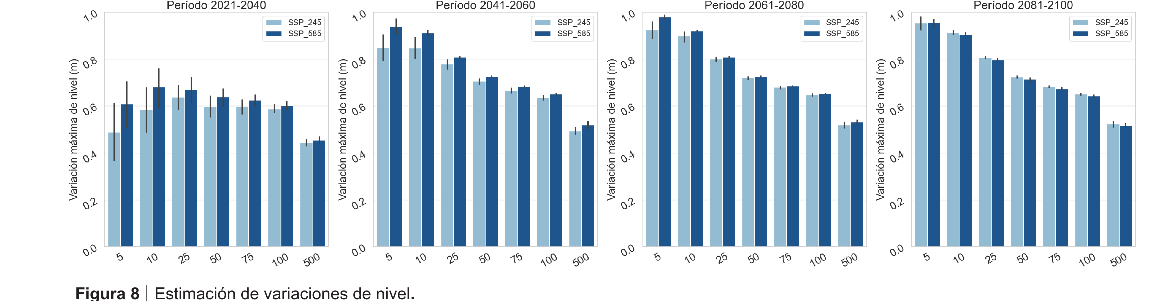
\includegraphics[width=\linewidth]{figures/fig_tanganika_variaciones_nivel}
  \caption{Variación máxima de nivel del Lago Tanganica respecto al histórico (m) para períodos de retorno de 5 a 500 años, en cuatro horizontes temporales (2021--2040, 2041--2060, 2061--2080, 2081--2100), bajo los escenarios SSP2-4.5 (azul claro) y SSP5-8.5 (azul oscuro). Las barras de error representan la incertidumbre del ensemble de 19 modelos CMIP6. El mayor incremento proyectado se alcanza en el período 2041--2060 para períodos de retorno cortos (T5--T10, $>$0,9 m); hacia finales del siglo los incrementos se estabilizan por debajo de 0,6 m para T $\geq$ 100 años. Figura reproducida de \parencite{navas2025tanganicaIA}.}
  \label{fig:tanganika_variaciones_nivel}
\end{figure}

\subsection{Conexión con HYDRA}

El caso Tanganica valida la cadena de cambio climático de \hydra en un contexto de escasa instrumentación y alta exposición: descarga de ERA5 y CMIP6, corrección de sesgo por método delta, generación sintética mediante bootstrap de residuos y análisis de extremos no paramétrico. Es la primera aplicación de la metodología a un sistema lacustre fuera de Europa, lo que demuestra la transferibilidad del enfoque a contextos con limitaciones de datos.

La combinación de regresión ML para estimar caudales a partir de variables climáticas, y de K-means para capturar la no linealidad de la respuesta del lago, es una extensión natural de los módulos de análisis estadístico de \hydra que no requiere modificar la arquitectura base del paquete.

\clearpage
\section{Vulnerabilidad de centrales hidroeléctricas andinas ante el cambio climático}
\label{sec:caso_andes}

\subsection{Contexto y problema}

La producción de energía hidroeléctrica en los países andinos ---Bolivia, Colombia, Ecuador y Perú--- depende de regímenes hidrológicos condicionados por la orografía de la cordillera, los patrones de precipitación estacional y los ciclos ENSO. La estimación de la vulnerabilidad de esta infraestructura frente al cambio climático requiere cubrir cuatro países, centenares de cuencas y varias décadas de proyecciones, con datos pluviométricos de calidad heterogénea y escasa cobertura en las zonas amazónicas \parencite{deljesus2019andean}. El caso pone a prueba la capacidad de los flujos de análisis de \hydra para gestionar datos de fuentes globales a escala regional.

\subsection{Metodología aplicada}

Los datos de precipitación proceden de las redes meteorológicas nacionales complementadas con la base de datos global NASA para cubrir las zonas de la Amazonia con escasa instrumentación. Los campos distribuidos se construyen mediante Kriging Universal con la elevación como variable de tendencia (MDT HydroSheds a 1~km de resolución). La validación cruzada produce una correlación media de Pearson $\rho = 0{,}42$, RMSE medio de 10,47 y sesgo medio del 8{,}0\% sobre el período 1981-2010. La temperatura y las variables de balance hídrico se extraen del reanálisis CFSR, con corrección del sesgo sistemático de $\approx -6\,^\circ$C respecto a las observaciones nacionales.

Las proyecciones climáticas proceden de 21 modelos GCM del proyecto CMIP5 bajo los escenarios RCP~4.5 y RCP~8.5 para los horizontes 2011-2040, 2041-2070 y 2071-2100. El modelo hidrológico VIC (Variable Infiltration Capacity), calibrado en estaciones de aforo seleccionadas por cobertura temporal, transforma los campos climáticos en series de caudal. La calibración en la estación de referencia CachEsperanz produce NSE $= 0{,}65$ y PBIAS $= 14{,}17\%$.

\subsection{Resultados}

Las proyecciones de precipitación muestran incrementos del $+15\%$ en el corto plazo hasta el $+20\%$ en el largo plazo bajo RCP~8.5 en la vertiente occidental, con decrementos del $5\%$--$15\%$ en el norte de Colombia y partes de Bolivia. Los cambios en temperatura son sistemáticamente positivos: entre $+1\,^\circ$C a corto plazo y $+3\,^\circ$C a largo plazo bajo RCP~8.5. Los cambios proyectados en caudal son no lineales respecto a los cambios de precipitación y presentan alta variabilidad estacional: en Perú y Ecuador bajo RCP~8.5 en el período 2071-2100, los caudales de los meses más húmedos aumentan más de un 40\% respecto al histórico, mientras que en Bolivia la respuesta puede ser moderada o incluso negativa en determinados meses. Las diferencias entre modelos GCM son el principal factor de incertidumbre en todos los países.

\begin{figure}[htbp]
  \centering
  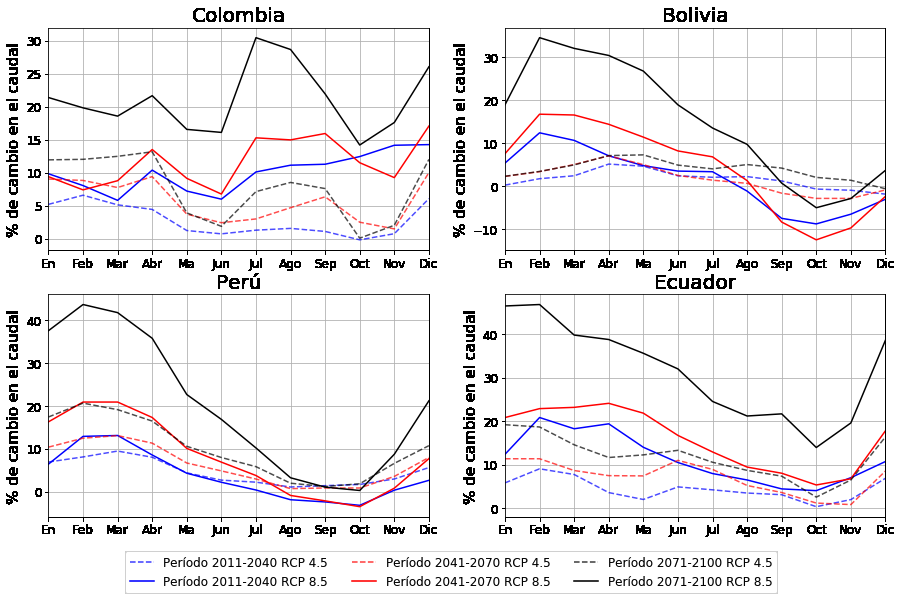
\includegraphics[width=\textwidth]{figures/fig_andes_caudales_cc.png}
  \caption{Influencia proyectada del cambio climático en el caudal mensual de Colombia, Bolivia, Perú y Ecuador para los escenarios RCP~4.5 y RCP~8.5 y tres horizontes temporales. Los cambios presentan una marcada variabilidad estacional y alcanzan valores superiores al $+40\%$ en Perú y Ecuador. Fuente: comunicación presentada en las VI Jornadas de Ingeniería del Agua \parencite{deljesus2019andean}.}
  \label{fig:andes_caudales_cc}
\end{figure}

\subsection{Conexión con HYDRA}

Este caso desarrolla tres capacidades que quedaron formalizadas en \hydra: la descarga automatizada de reanálisis y proyecciones globales (\path{pyhydra.data_sources.climate_change}), la interpolación de campos distribuidos con Kriging Universal y covariables topográficas (\path{pyhydra.climate.spatial_analysis}), y la corrección de sesgo mediante mapeo de cuantiles (\path{pyhydra.climate.bias_correction}). La escala regional ---cuatro países, más de 200 subcuencas, 21 modelos GCM--- anticipa la arquitectura de procesamiento masivo que \hydra formaliza con APIs uniformes por fuente de datos y módulo de análisis.

\clearpage
\section{Impacto de las decisiones metodológicas en el riesgo de inundación bajo cambio climático}
\label{sec:caso_iahr2022}

\subsection{Contexto y problema}

La práctica convencional asigna directamente el período de retorno de la precipitación al caudal pico obtenido a partir del hietograma de diseño correspondiente. Esta transferencia es conceptualmente incorrecta en cuencas no lineales, donde la distribución de probabilidad del impacto hidráulico no coincide con la del forzamiento meteorológico. El trabajo de \textcite{deljesus2022iahr}, presentado en el 39th IAHR World Congress (Granada, 2022), cuantifica sistemáticamente la diferencia entre esta aproximación estándar y la metodología estocástica de \hydra en una cuenca del norte de España con régimen hidrológico atlántico, bajo distintos escenarios y horizontes de cambio climático.

\subsection{Metodología aplicada}

El estudio emplea 15 modelos del conjunto EURO-CORDEX bajo los escenarios RCP~4.5 y RCP~8.5, con corrección de sesgo mediante mapeo de cuantiles empírico sobre el período histórico de referencia \parencite{teutschbein2012biascorrection}. Los eventos de crecida se caracterizan por caudal pico, duración y forma del hidrograma (clasificada mediante k-means), y la dependencia multivariante se modela con cópulas gaussianas. A partir de la distribución ajustada se generan 10.000 años de eventos sintéticos, de los que se seleccionan 200 casos representativos mediante el algoritmo de máxima disimilitud para su simulación hidráulica completa con Iber en régimen no permanente. Los calados del resto de eventos se reconstruyen con el emulador k-NN. El análisis de extremos se aplica directamente sobre la variable hidráulica (calado) y no sobre la precipitación forzante.

\subsection{Resultados}

La diferencia entre la metodología estocástica y la estándar es sistemática y significativa en todos los períodos de retorno, escenarios y horizontes. La \cref{tab:iahr2022_caudales} recoge los caudales de diseño para los cuatro períodos de retorno y los seis escenarios-horizonte. Los caudales de la metodología estocástica son entre un 30\% y un 37\% superiores en todos los casos.

\begin{table}[htbp]
  \centering
  \caption{Caudales de diseño (m\textsuperscript{3}/s) estimados con la metodología estocástica de \hydra y la metodología estándar basada en curvas IDF, para cuatro períodos de retorno, dos escenarios de cambio climático y tres horizontes temporales. La diferencia entre enfoques es del 30--37\% en todos los casos. Fuente: \parencite{deljesus2022iahr}.}
  \label{tab:iahr2022_caudales}
  \resizebox{\textwidth}{!}{%
  \begin{tabular}{llrrrr}
    \toprule
    Escenario & Metodología & $T$ (años) & 2011--2040 & 2041--2070 & 2071--2100 \\
    \midrule
    \multirow{8}{*}{RCP~4.5}
      & \multirow{4}{*}{Estocástica}
        & 50  & 249,9 & 257,1 & 265,7 \\
      & & 100 & 278,5 & 286,6 & 296,8 \\
      & & 200 & 317,3 & 326,8 & 339,2 \\
      & & 500 & 362,3 & 373,5 & 388,4 \\
    \cmidrule{2-6}
      & \multirow{4}{*}{Estándar (IDF)}
        & 50  & 187,4 & 192,8 & 199,3 \\
      & & 100 & 208,8 & 214,9 & 222,6 \\
      & & 200 & 238,0 & 245,1 & 254,4 \\
      & & 500 & 271,7 & 280,1 & 291,3 \\
    \midrule
    \multirow{8}{*}{RCP~8.5}
      & \multirow{4}{*}{Estocástica}
        & 50  & 258,8 & 262,5 & 271,2 \\
      & & 100 & 288,7 & 293,0 & 303,1 \\
      & & 200 & 329,4 & 334,7 & 346,7 \\
      & & 500 & 376,7 & 383,0 & 397,4 \\
    \cmidrule{2-6}
      & \multirow{4}{*}{Estándar (IDF)}
        & 50  & 194,1 & 196,9 & 203,4 \\
      & & 100 & 216,5 & 219,8 & 227,3 \\
      & & 200 & 247,1 & 251,0 & 260,0 \\
      & & 500 & 282,5 & 287,3 & 298,1 \\
    \bottomrule
  \end{tabular}}
\end{table}

Los mapas de inundación resultantes no son proporcionales a la diferencia en caudales, lo que evidencia la no linealidad del sistema y descarta cualquier factor de corrección simple aplicable a los resultados de la metodología estándar. La diferencia entre enfoques es mayor que la incertidumbre intermodelo de los escenarios climáticos para todos los períodos de retorno considerados.

\begin{figure}[htbp]
  \centering
  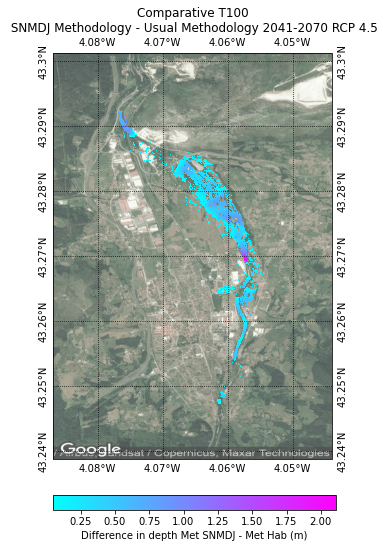
\includegraphics[height=0.58\textheight]{figures/fig_iahr2022_comparativa.png}
  \caption{Diferencia espacial de calado para $T = 100$ años entre la metodología estocástica y la metodología habitual bajo RCP~4.5 en el horizonte 2041--2070. La distribución espacial confirma que la discrepancia entre enfoques no puede representarse mediante un factor uniforme sobre el caudal. Fuente: presentación del 39th IAHR World Congress \parencite{deljesus2022iahr}.}
  \label{fig:iahr2022_mapas}
\end{figure}

\subsection{Conexión con HYDRA}

Este trabajo proporciona la primera validación cuantitativa del error sistemático introducido por la metodología estándar en estudios de inundación bajo cambio climático. Los módulos validados son los mismos que los del Besaya y Calle 30: corrección de sesgo (\texttt{pyhydra.climate.bias\_correction}), generación estocástica con cópulas (\texttt{pyhydra.climate.spatial\_analysis}), selección por máxima disimilitud (\texttt{pyhydra.climate.hybrid\_downscaling}) y reconstrucción k-NN del dominio hidráulico. La conclusión de que la elección de metodología es una fuente de incertidumbre de primer orden sustenta la hipótesis central de la tesis: la metodología estocástica basada en impactos no es un refinamiento opcional, sino una condición para obtener estimaciones de riesgo no sesgadas.

\clearpage
\section{SIMPCCe: aportaciones a embalses bajo cambio climático}
\label{sec:caso_simpce}

\subsection{Contexto y problema}

El cambio climático puede reducir sistemáticamente las aportaciones disponibles en épocas de estiaje en las cuencas españolas, comprometiendo el suministro en sistemas regulados. Cuantificar este impacto requiere combinar reanálisis histórico, proyecciones de modelos climáticos, corrección de sesgo y modelización hidrológica sobre cualquier punto de la red hídrica nacional. SIMPCCe responde a esa necesidad mediante una cadena Python para evaluar aportaciones a embalses bajo escenarios climáticos, desarrollada en el marco de la guía metodológica de Fundación Canal para la estimación de aportaciones mínimas a embalses en el contexto de cambio climático \parencite{fundacioncanal2022guiaembalses}. La herramienta fue presentada en JIA 2023 \parencite{navas2023simpce} y en el congreso europeo de IAHR de 2024 \parencite{navas2024iahrsimpcce}, y publicada posteriormente como artículo en \textit{Ingeniería del Agua} \parencite{navas2025simpce}, una de las publicaciones que integran el compendio de resultados de esta tesis. La aplicación integra módulos climáticos de \pyhydra en un flujo orientado a gestores del recurso hídrico; además, el Observatorio del Agua de la Fundación Botín reconoció el trabajo con el Premio al Talento Joven ``M.R. Llamas''.

\subsection{Metodología aplicada}

SIMPCCe consta de cinco módulos que se corresponden directamente con capacidades de \hydra. El primero descarga automáticamente datos de precipitación y temperatura del conjunto SPAIN02~v5 \parencite{herrera2016spain02} y aportaciones del modelo SIMPA-CEDEX para el período 1950-2015, junto con 10 modelos del proyecto CORDEX-AEMET bajo los escenarios RCP~4.5 y RCP~8.5 para tres horizontes temporales. El segundo delimita la cuenca aportante al punto de interés a partir de un MDT de 200~m y extrae la malla de puntos climáticos distribuidos. El tercero entrena una red neuronal artificial (ANN) sobre las componentes principales de la precipitación y temperatura distribuidas (PCA al 95\% de la varianza, división 80/20 entrenamiento/validación) para predecir las aportaciones mensuales. El cuarto aplica la corrección de sesgo SDM \parencite{switanek2017sdm} a cada combinación modelo-escenario-horizonte, generando 60 series corregidas por variable (10 modelos $\times$ 2 escenarios $\times$ 3 períodos). El quinto simula 20 series futuras de aportaciones con la ANN entrenada y sintetiza los resultados en informes automáticos con estadísticas anuales, SPI e índices de fiabilidad para la toma de decisiones.

\subsection{Resultados}

Las conclusiones del análisis a escala nacional con 10 modelos CORDEX confirman que el cambio climático reduce sistemáticamente las aportaciones medias anuales en la mayoría de las cuencas españolas, que las aportaciones mínimas en épocas de estiaje disminuyen incluso en cuencas donde la precipitación media no registra cambios estadísticamente significativos, y que la sequía hidrológica tiende a aumentar en severidad y duración bajo ambos escenarios. La envolvente intermodelo permite cuantificar la incertidumbre y orientar decisiones de planificación con distintos niveles de cautela.

\begin{figure}[htbp]
  \centering
  \begin{subfigure}[t]{0.47\textwidth}
    \centering
    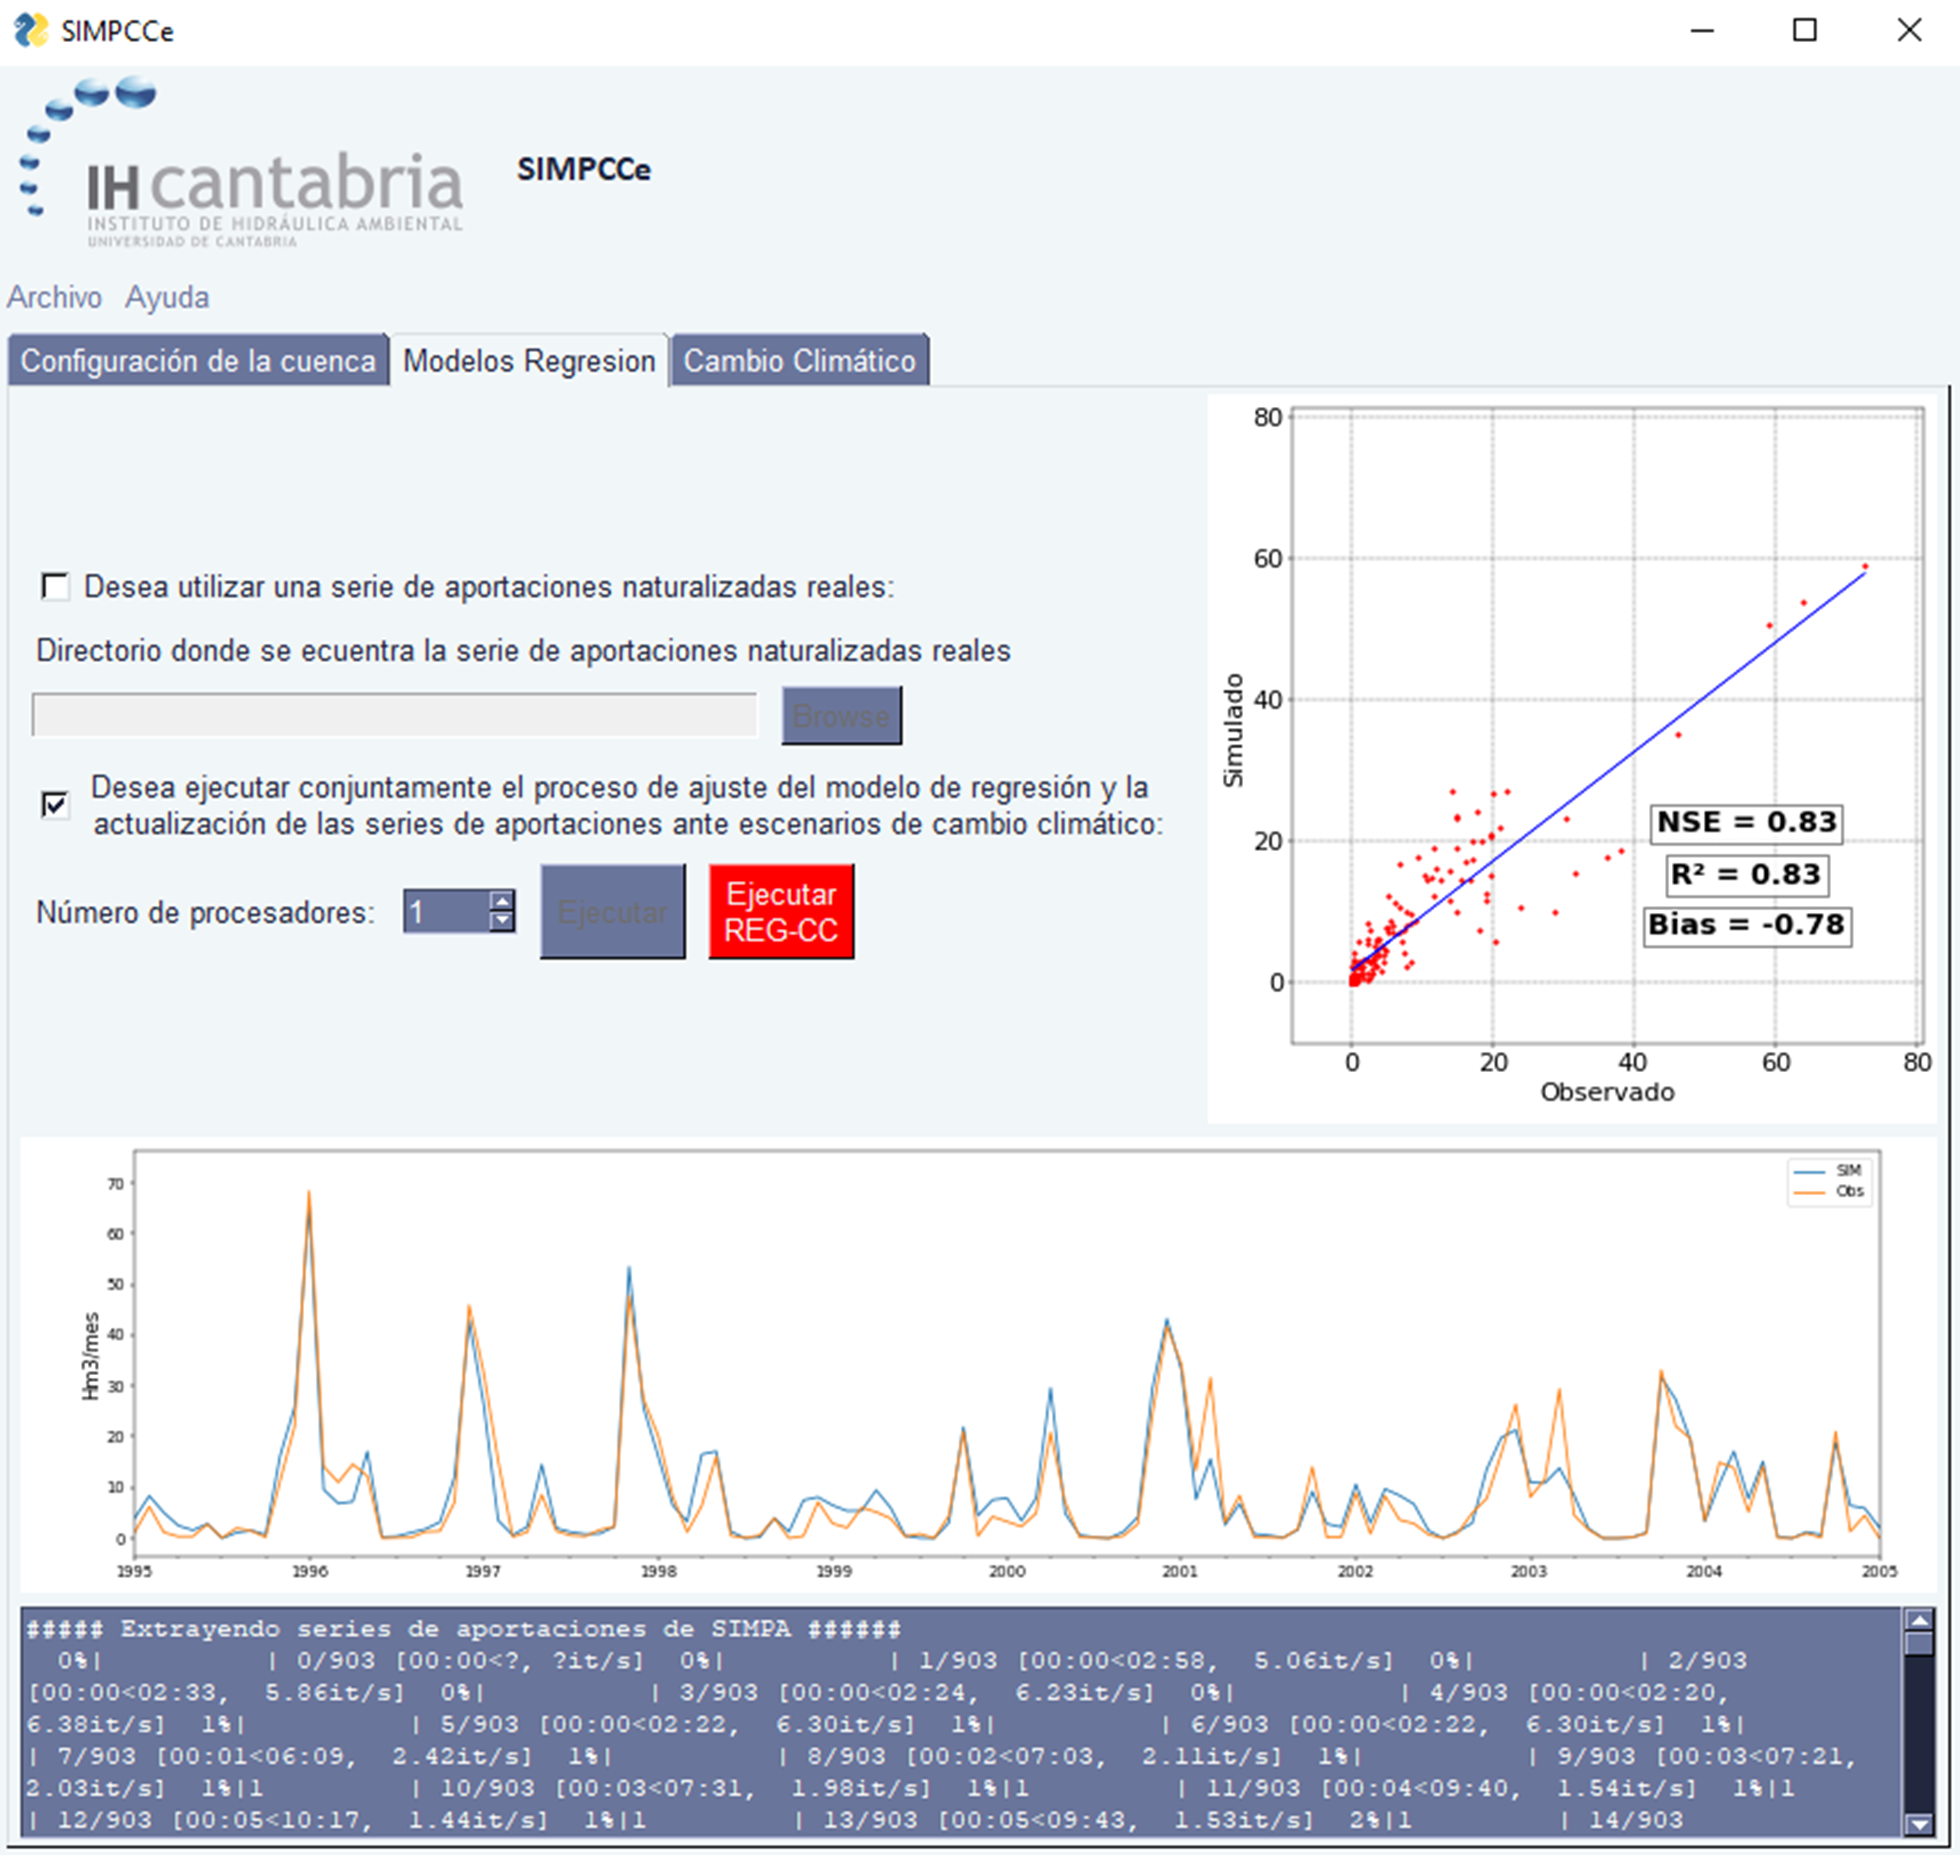
\includegraphics[width=\textwidth]{figures/fig_simpcce_interfaz.png}
    \caption{Interfaz de entrenamiento y validación.}
  \end{subfigure}
  \hfill
  \begin{subfigure}[t]{0.50\textwidth}
    \centering
    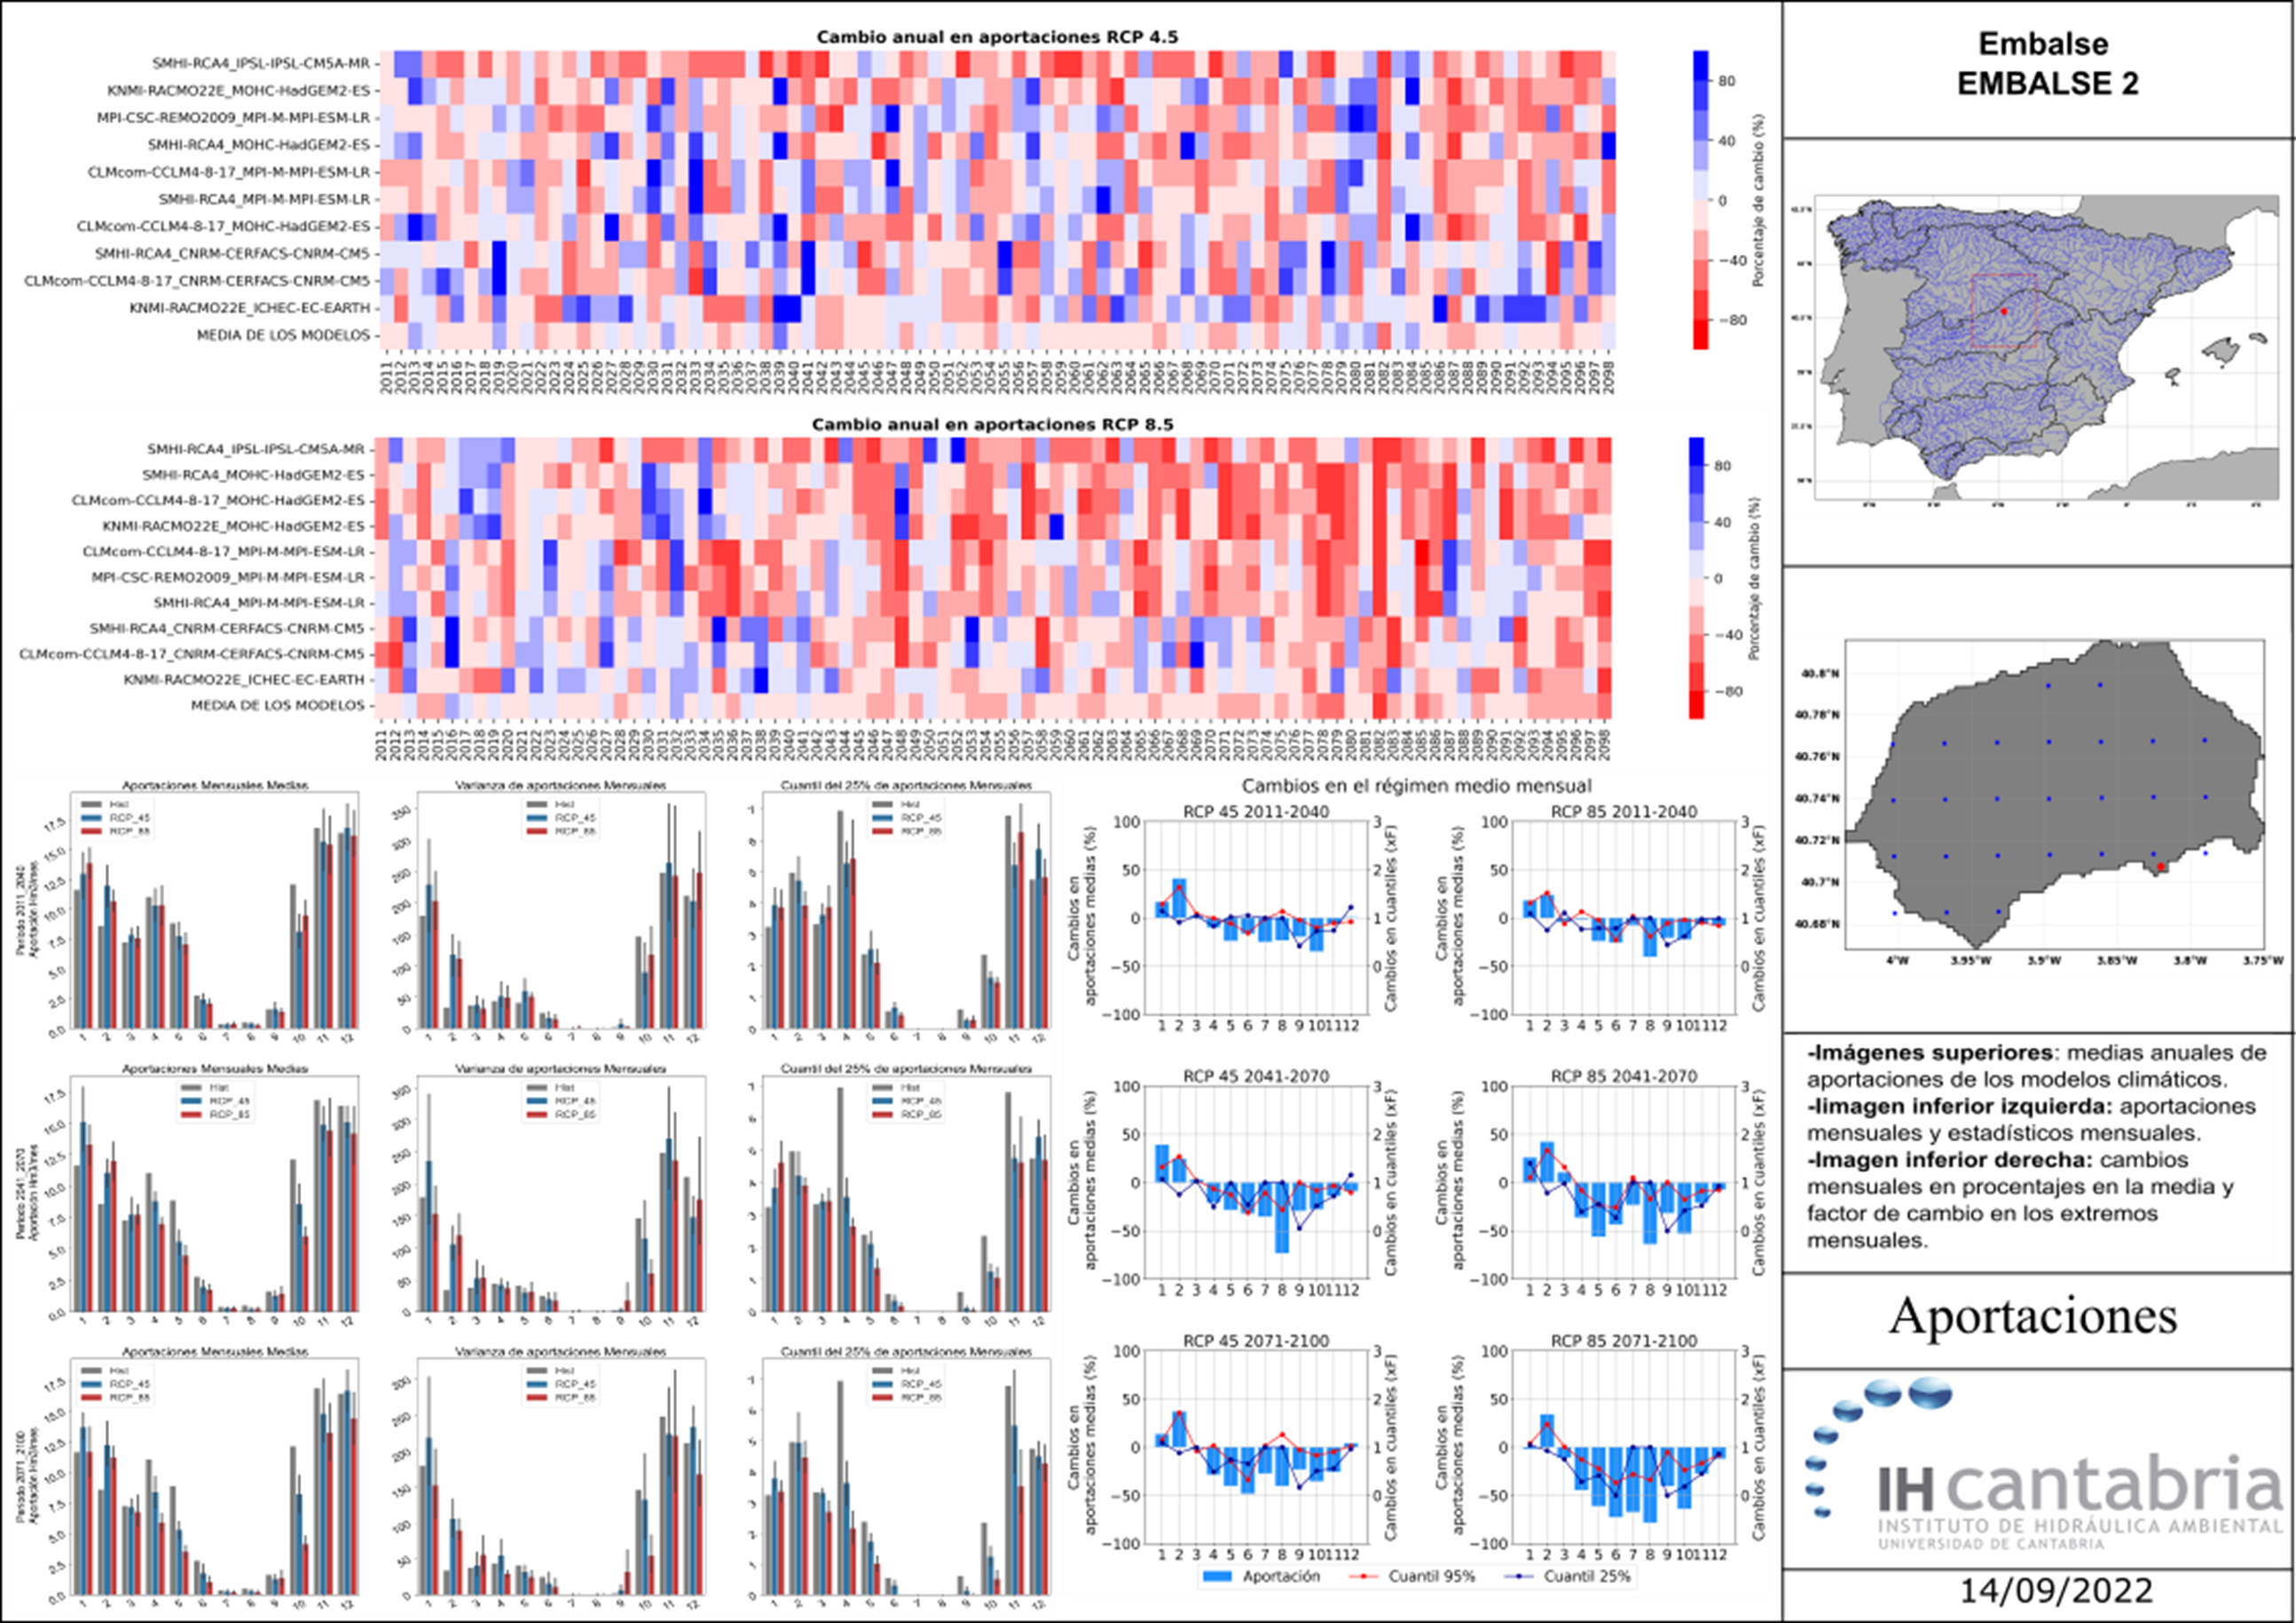
\includegraphics[width=\textwidth]{figures/fig_simpcce_resultados.png}
    \caption{Ficha automática de cambio en aportaciones.}
  \end{subfigure}
  \caption{Productos operativos de SIMPCCe. La interfaz permite ejecutar la cadena de cálculo y validar la red neuronal; las fichas sintetizan los cambios anuales y mensuales bajo RCP~4.5 y RCP~8.5, junto con la incertidumbre intermodelo. Fuentes: presentaciones JIA 2023 e IAHR Europe 2024 \parencite{navas2023simpce,navas2024iahrsimpcce}.}
  \label{fig:simpce_output}
\end{figure}

\subsection{Conexión con HYDRA}

SIMPCCe es el caso de uso más completo del bloque de cambio climático de \hydra: los módulos \texttt{pyhydra.data\_sources.climate\_change}, \texttt{pyhydra.climate.bias\_correction} y \texttt{pyhydra.climate.time\_series} operan integrados como una cadena de cálculo. La conexión de la herramienta con la guía metodológica para la estimación de aportaciones mínimas a embalses promovida por Fundación Canal \parencite{fundacioncanal2022guiaembalses} ilustra la dimensión industrial de la investigación y su transferencia a problemas reales de planificación de recursos hídricos.

\clearpage
\section{Atlas de Riesgo Climático de la República de Panamá}
\label{sec:caso_panama}

\subsection{Contexto y problema}

El Atlas Interactivo de Riesgo Climático de Panamá \parencite{ihcantabria2023panama} es la aplicación de mayor escala geográfica realizada con las herramientas de \hydra. El proyecto, encargado por la Dirección de Cambio Climático del Ministerio de Ambiente y financiado por el Banco Interamericano de Desarrollo, abarca las 52 cuencas hidrológicas del país ---18 en la vertiente caribe y 34 en la del Pacífico--- con superficies individuales de hasta 13.400~km\textsuperscript{2}. El proyecto cuantifica de forma integrada los riesgos climáticos para los horizontes 2030, 2050 y 2070 bajo los escenarios SSP2-4.5 y SSP5-8.5, incluyendo inundación fluvial en las 52 cuencas, inundación costera en 1.464 puntos de ambas costas, y viento extremo sobre el área metropolitana de Ciudad de Panamá.

\subsection{Metodología aplicada}

La cadena metodológica moviliza los tres bloques funcionales de \hydra en una ejecución a escala nacional. El bloque de datos descarga ERA-5 \parencite{hersbach2020era5}, precipitación TRMM/TMPA \parencite{huffman2007trmm} y proyecciones de 23 modelos CMIP6 \parencite{eyring2016cmip6} bajo SSP2-4.5 y SSP5-8.5 para el período 1950-2100. NEOPRENE \parencite{diezsierra2023neoprene}, mediante sus generadores NSRP/STNSRP, rellena los huecos en 73 estaciones meteorológicas nacionales para el período 1950-2022. Los campos de precipitación se interpolan a malla de 1~km mediante Kriging Universal con elevación y precipitación media TRMM como covariables.

La corrección de sesgo se ejecuta en 414 combinaciones (23 modelos $\times$ 2 escenarios $\times$ 6 variables $\times$ 3 períodos) mediante QDM para precipitación \parencite{cannon2015sdm} y SDM para temperatura \parencite{switanek2017sdm}. El modelo hidrológico LEM ---calibrado con Nash-Sutcliffe NS $= 0{,}87$ en las estaciones de referencia--- simula los caudales en 200-300 subcuencas; los caudales máximos para períodos de retorno de 10, 50 y 100 años se calculan con ajuste GEV mediante \texttt{pyhydra.climate.time\_series.extremes}. Las manchas de inundación fluvial se generan con el modelo SFINCS para el conjunto nacional y con modelos hidráulicos 2D de alta resolución para el área metropolitana.

\subsection{Resultados}

El atlas publica seis familias de capas de riesgo en un visor web interactivo del Ministerio de Ambiente. Las capas de inundación fluvial cubren las 52 cuencas para tres períodos de retorno ($T = 10, 50, 100$ años) y tres horizontes temporales bajo dos escenarios SSP. Las capas de inundación costera comprenden 52 escenarios de nivel de agua total en los 1.464 puntos costeros analizados a lo largo de ambas costas. Las proyecciones de índices climáticos extremos (SPI, SPEI, RX1, RX5 y otros) se calculan para los tres horizontes temporales. La dimensión operativa del proyecto ---23 modelos GCM, 414 correcciones de sesgo, 200-300 subcuencas, miles de simulaciones SFINCS--- ilustra la capacidad de \hydra para ejecutar flujos de análisis masivos sin modificar la arquitectura base del sistema.

\begin{figure}[htbp]
  \centering
  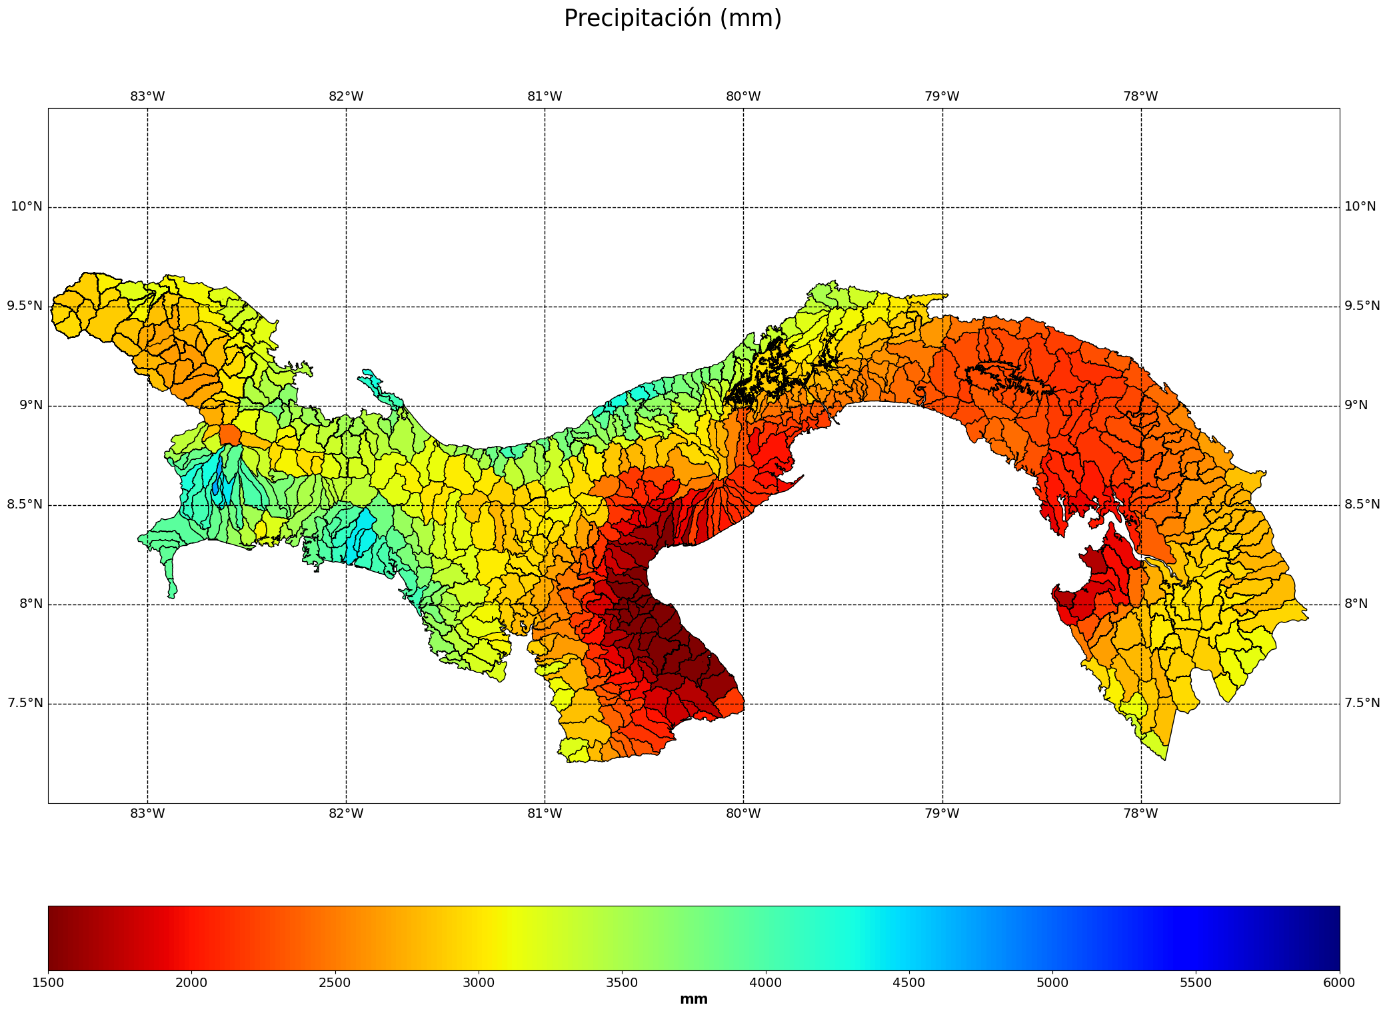
\includegraphics[width=\textwidth]{figures/fig_panama_precipitacion.png}
  \caption{Precipitación media distribuida por subcuencas para la República de Panamá, obtenida mediante el flujo nacional de descarga, control de calidad e interpolación espacial que alimenta los modelos hidrológicos y las ejecuciones masivas de SFINCS. Fuente: memoria técnica del Atlas de Riesgo Climático de Panamá \parencite{ihcantabria2023panama}.}
  \label{fig:panama_atlas}
\end{figure}

\subsection{Conexión con HYDRA}

El Atlas de Panamá es la aplicación más amplia de \hydra en un contexto de encargo industrial a escala nacional. El proyecto fue el primer banco de pruebas a gran escala del bloque de datos (\texttt{pyhydra.data\_sources}) para la descarga y procesamiento de ERA-5, CMIP6 y datos TRMM; del módulo de corrección de sesgo (\texttt{pyhydra.climate.bias\_correction}) para el procesamiento masivo de 23 modelos y 6 variables; y de la interfaz SFINCS (\texttt{pyhydra.modeling.hydraulic.sfincs}) para la generación sistemática de manchas de inundación a escala de país. Los patrones de automatización y reutilización de configuración validados en este proyecto se trasladaron directamente a la arquitectura final de \hydra.

\clearpage
\section{Síntesis de la validación}
\label{sec:sintesis_validacion}

\subsection{Cobertura de módulos}

Los nueve casos de estudio cubren conjuntamente todos los módulos de \hydra a distintas escalas, regímenes hidrológicos y contextos institucionales. La \cref{tab:validacion_modulos} resume la correspondencia entre casos y módulos validados.

\begin{table}[htbp]
  \centering
  \caption{Cobertura de módulos de \pyhydra por caso de estudio.}
  \label{tab:validacion_modulos}
  \small
  \begin{tabular}{>{\raggedright\arraybackslash}p{0.24\textwidth}>{\raggedright\arraybackslash}p{0.64\textwidth}}
    \toprule
    Caso & Módulos validados \\
    \midrule
    Mallorca & SIAR, PERSIANN/TRMM como diagnóstico, kriging espacial, cópulas gaussianas, MaxDiss, k-NN, downscaling híbrido desde lluvia; simulación hidráulica con Iber (herramienta externa, sin adaptador en \pyhydra) \\
    Besaya & Extremos de caudal, cópulas gaussianas, HEC-RAS/SFINCS en desarrollos posteriores \parencite{navas2018besaya}; Iber como motor hidráulico externo en la aplicación inicial de 2018 \\
    Calle 30 & ERA5, extremos precipitación, cópulas multivariantes, HEC-HMS, HEC-RAS 1D, downscaling híbrido, períodos de retorno por pixel \\
    Valencia 2024 & AEMET/SIAR/AVAMET, GEV (MLE, L-momentos, MCMC con PyMC), RFA, cuantificación de incertidumbre \\
    Tanganica & ERA5, CMIP6, corrección de sesgo delta, regresión ML (AdaBoost), K-means, bootstrap sintético, extremos no paramétricos \\
    Andes (Bolivia, Colombia, Ecuador, Perú) & Kriging Universal con MDT global, CMIP5, corrección de sesgo, modelo VIC \\
    Cuenca atlántica -- CC (IAHR 2022) & EURO-CORDEX, corrección de sesgo, cópulas gaussianas, MaxDiss, k-NN, comparación metodologías; simulación hidráulica con Iber (herramienta externa) \\
    SIMPCCe & SPAIN02, CORDEX-AEMET, corrección de sesgo SDM, ANN, análisis de sequía, informes automáticos \\
    Atlas Panamá & ERA5, TRMM, CMIP6, NEOPRENE (NSRP/STNSRP), kriging 1~km, 414 correcciones SDM/QDM, GEV, SFINCS, inundación costera \\
    \bottomrule
  \end{tabular}
\end{table}

\subsection{Escala computacional gestionada}

Un indicador directo del beneficio industrial de la automatización es la escala de cálculo que cada caso gestionó sin intervención manual entre etapas. La \cref{tab:escala_computacional} recoge las magnitudes documentadas en los casos; ninguna de estas campañas habría sido operativamente viable con flujos manuales de configuración, ejecución y postprocesado caso a caso. A ellas se añade la reducción del 94\% del coste de cálculo de períodos de retorno conjuntos lograda por el emulador GPR en la línea de extensión multivariante \parencite{urrea2026vine}.

\begin{table}[htbp]
  \centering
  \caption{Indicadores de escala computacional gestionada automáticamente en los casos de estudio.}
  \label{tab:escala_computacional}
  \small
  \begin{tabular}{>{\raggedright\arraybackslash}p{0.24\textwidth}>{\raggedright\arraybackslash}p{0.64\textwidth}}
    \toprule
    Caso & Escala gestionada por la cadena automatizada \\
    \midrule
    Besaya (rugosidad) & Ensemble emparejado de 995 realizaciones de Manning ejecutado en dos motores hidráulicos 2D (1\,990 simulaciones), con carga, georreferenciación y análisis conjunto de todas las salidas \\
    Calle 30 & Miles de eventos sintéticos multisitio; subconjunto representativo simulado en HEC-HMS y HEC-RAS 1D y reconstrucción k-NN del resto sobre la red de túneles \\
    Mallorca & Miles de eventos sintéticos de precipitación; reconstrucción k-NN (6 vecinos) de calados y velocidades del conjunto no simulado \\
    Atlas de Panamá & 414 correcciones de sesgo SDM/QDM, interpolación climática nacional a 1~km, 200--300 subcuencas y ejecución sistemática de SFINCS a escala de país \\
    SIMPCCe & 60 series corregidas por variable (10 modelos $\times$ 2 escenarios $\times$ 3 horizontes) y 20 realizaciones futuras por punto de la red hídrica nacional \\
    Tanganica & 19 modelos CMIP6 bajo dos escenarios SSP con downscaling estadístico y remuestreo bootstrap \\
    \bottomrule
  \end{tabular}
\end{table}

\subsection{Transferencia y reproducibilidad}

La existencia de publicaciones para cada caso proporciona referencias externas independientes. Los 26 notebooks generales de ejemplo permiten repetir funcionalidades de \hydra con datos abiertos, sintéticos controlados o modelos oficiales de referencia, mientras que las 23 entradas de casos piloto del catálogo web documentan flujos territoriales completos. El material interno utilizado para preparar artículos, incluido el análisis de sensibilidad de Manning, se mantiene separado del catálogo general y se utiliza en este capítulo únicamente como fuente de resultados científicos del caso correspondiente.

\subsection{Limitaciones observadas}

A lo largo de los casos se han identificado tres categorías de limitaciones. Las limitaciones de datos afectan a la longitud y homogeneidad de las series disponibles. Las limitaciones computacionales derivan de la dependencia de modelos externos que requieren instalaciones específicas o tiempos de cálculo prolongados. Las limitaciones metodológicas están asociadas a la hipótesis de estacionariedad de los generadores estocásticos. Ninguna invalida la arquitectura de \hydra, pero todas se documentan en los notebooks correspondientes para que el usuario pueda evaluar su alcance antes de aplicar la herramienta a un nuevo caso.

La validación realizada no debe entenderse como una validación universal de todos los módulos en todos los contextos posibles, sino como una validación operativa de la arquitectura mediante casos que ejercitan combinaciones representativas de módulos, datos y motores externos. Los nueve casos no son experimentos homogéneos comparables entre sí, sino instancias complementarias cuya diversidad geográfica, de escala y de fenómeno es precisamente la que garantiza la generalidad funcional de \hydra.
